% start the document

% specify the document layout and font size
\documentclass[preprint,12pt]{elsarticle}
% \documentclass[final,twocolumn,12pt]{elsarticle}
% \usepackage[margin=1.5cm,includefoot]{geometry}
\usepackage{setspace}

% uploading packages
\usepackage{graphicx}
\usepackage{amssymb}
\usepackage{textcomp} % https://latex.org/forum/viewtopic.php?f=4&t=3364#p13124, https://tex.stackexchange.com/questions/165115
\usepackage{gensymb}
\usepackage{lineno}
\usepackage{mathtools}
\usepackage[title]{appendix}
\usepackage{pgfmath}
\newcommand{\calcnum}[1]{%
    \pgfmathparse{#1}%
    \num[round-mode=places,round-precision=1]{\pgfmathresult}%
}
\usepackage[separate-uncertainty=true]{siunitx} % \usepackage{xr-hyper} %needs to  be before hyperref
\usepackage{xurl} %needs to be before hyperref
\usepackage[colorlinks]{hyperref}
\hypersetup{breaklinks=true} % set automatically by hyperref?
% \PassOptionsToPackage{hyphens}{url}\usepackage{hyperref} %allow URLs to break across lines
\usepackage[nameinlink,capitalise]{cleveref} %needs to appear after hyperref, https://tex.stackexchange.com/questions/396728/my-equations-referencing-not-working
\Crefname{figure}{Figure}{Figures} %needs to appear after hyperref and cleveref
\crefname{appsec}{Appendix}{Appendices}
\newcommand\crefrangeconjunction{--} % modify the reference style
\usepackage{mathrsfs}
\usepackage{enumitem}
\usepackage{tabulary}
\usepackage{caption}
\usepackage{subcaption}
\usepackage{multirow}
\usepackage{makecell} % https://tex.stackexchange.com/questions/2441/how-to-add-a-forced-line-break-inside-a-table-cell
\newcommand{\NA}{---} % holds an m-dash
\graphicspath{{figures/}} %Setting the graphicspath
% ---------to deal with the double quotes----------- 
\usepackage [english]{babel}
\usepackage [autostyle, english = american]{csquotes}
\MakeOuterQuote{"}
\usepackage{listings}[breakatwhitespace=true,escapechar=\%]
\usepackage{matlab-prettifier}
\newcommand{\matlab}[1]{\mbox{\lstinline[style=Matlab-editor]{#1}}}
%alternatively can use `` '' format for double quotes
\usepackage{booktabs}
\setlength{\abovetopsep}{1ex}
\usepackage[shortcuts,abbreviations]{glossaries-extra}
\newcommand*{\TCac}[1]{\ecapitalisewords{\glsentrylong{#1}}}
% remove the "Preprint submitted to Elsevier" footer on the first page
\makeatletter
\def\ps@pprintTitle{%
   \let\@oddhead\@empty
   \let\@evenhead\@empty
   \def\@oddfoot{\reset@font\hfil\thepage\hfil}
   \let\@evenfoot\@oddfoot
}
\makeatother

% Cross referencing with the xr package in Overleaf (https://www.overleaf.com/learn/how-to/Cross_referencing_with_the_xr_package_in_Overleaf)
\makeatletter
\newcommand*{\addFileDependency}[1]{% argument=file name and extension
  \typeout{(#1)}
  \@addtofilelist{#1}
  \IfFileExists{#1}{}{\typeout{No file #1.}}
}
\makeatother
\newcommand*{\myexternaldocument}[1]{%
    \externaldocument{#1}%
    \addFileDependency{#1.tex}%
    \addFileDependency{#1.aux}%
}

\usepackage{nameref,zref-xr}
\zxrsetup{toltxlabel}
%https://tex.stackexchange.com/questions/77774/undefined-control-sequence-when-cross-referencing-with-xr-hyper
% \myexternaldocument{supp}

\biboptions{sort&compress}
\interfootnotelinepenalty=10000 %prevent footnotes from getting split across columns/pages 
%\patchcmd{\emailauthor}{(#2)}{(S.G. Baird).}{}{} %Removes/Abbreviates corresponding author name after Email address so that the footnote doesn't take up 2 lines.
% Double Spacing
% \doublespacing
\usepackage[margin=1.5cm,includefoot]{geometry}
\usepackage{auto-paper}
% \PassOptionsToPackage{refcheck}{auto-paper} %comment this out before submission

\zexternaldocument*{main-frankenstein-1} %try deleting log files if producing an error, see https://tex.stackexchange.com/questions/131709/unclean-aux-file-causes-file-ended-while-scanning-use-of-newlbel-error-wh
% Concatenate the different "values" .tex files
%RMSE values
% \newcommand{\baryrmse}{0.0242}
% \newcommand{\gprrmse}{0.0220}
% \newcommand{\idwrmse}{0.0345}
% \newcommand{\nnrmse}{0.0448}
% \newcommand{\avgrmse}{0.1302}
% %paper-data6
% \newcommand{\baryrmse}{0.0238}
% \newcommand{\gprrmse}{0.0218}
% \newcommand{\idwrmse}{0.0356}
% \newcommand{\nnrmse}{0.0445}
% \newcommand{\avgrmse}{0.1283}
%\newcommand{\gprrmsePercReduction}{83}
% paper-data9
\newcommand{\baryrmse}{0.0239}
\newcommand{\gprrmse}{0.0217}
\newcommand{\idwrmse}{0.0343}
\newcommand{\nnrmse}{0.0448}
\newcommand{\avgrmse}{0.1284}
\newcommand{\gprrmsePercReduction}{83.1}

%MAE values
% \newcommand{\barymae}{0.0145}
% \newcommand{\gprmae}{0.0145}
% \newcommand{\idwmae}{0.0223}
% \newcommand{\nnmae}{0.0307}
% \newcommand{\avgmae}{0.0965}
% %paper-data6
% \newcommand{\barymae}{0.0145}
% \newcommand{\gprmae}{0.0145}
% \newcommand{\idwmae}{0.0225}
% \newcommand{\nnmae}{0.0307}
% \newcommand{\avgmae}{0.0955}
%paper-data9
\newcommand{\barymae}{0.0145}
\newcommand{\gprmae}{0.0145}
\newcommand{\idwmae}{0.0223}
\newcommand{\nnmae}{0.0308}
\newcommand{\avgmae}{0.0959}

%\newcommand{\nnomega}{2.8709 \pm 0.69112}
\newcommand{\nnomega}{2.8702 \pm 0.69117}

\newcommand{\symtime}{76}

\newcommand{\nigprbrkrmse}{0.1471}

%Supplementary
\newcommand{\thr}{\SI{1.1}{\joule\per\square\meter}}
\newcommand{\sigthr}{\SI{1.1}{\joule\per\square\meter}}
\newcommand{\thrtwo}{\SI{1.2}{\joule\per\square\meter}}


%% main-frankenstein-2
\newcommand{\minsymdist}{$\sim$\SI{64.0}{\tobydeg}}
\newcommand{\percExplained}{$\sim$\SI{99.6}{\percent}}
\newcommand{\percFiveVsOne}{$\sim$\SI{70}{\percent}}
\newcommand{\dimOne}{$\sim$\SI{65}{\tobydeg}}

% figure info, etc. that can dynamically change (color of points, etc.)
\newcommand{\startpt}{red points}
\newcommand{\singlept}{magenta points}
\newcommand{\sympt}{dark blue points}
\newcommand{\singlesympt}{dark blue point}
\newcommand{\refpt}{white circle}
\newcommand{\vbordercolor}{black}
\newcommand{\vcellcolor}{light blue}
\newcommand{\inpt}{input}
\newcommand{\outpt}{prediction}
% \newcommand{\inptvar}{ninputpts}
% \newcommand{\distfn}{GBdist4}
\newcommand{\vfzorepo}{\gls{vfz} repository}
\newcommand{\mytitleone}{Five Degree-of-Freedom Property Interpolation of Arbitrary Grain Boundaries via \glsentrytitlecase{vfz}{long} Framework}
% \newcommand{\mytitletwo}{Properties of a \glsentrytitlecase{5dof}{long} \glsentrytitlecase{fz}{long} defined via \glsentrytitlecase{vfz}{long} Framework}
\newcommand{\mytitletwo}{$O_h$ \glsentrytitlecase{5dof}{long} \glsentrytitlecase{fz}{long} Properties via \glsentrytitlecase{vfz}{long} Framework}
\makeglossaries
\GlsXtrEnableEntryCounting{abbreviation}{3}
% \glssetcategoryattribute{abbreviation}{indexonlyfirst}{true}
\glssetcategoryattribute{abbreviation}{nohyper}{true}

% \setabbreviationstyle[abbreviation]{long-short}

% \glsenableentrycount
% \glssetcategoryattribute{abbreviation}{entrycount}{2}

\newabbreviation[longplural=five degrees of freedom]{5dof}{5DOF}{five degree-of-freedom}
\newabbreviation[longplural=three degrees of freedom]{3dof}{3DOF}{three degree-of-freedom}
\newabbreviation[longplural=degrees of freedom]{dof}{DOF}{degree of freedom}
\newabbreviation{ebsd}{EBSD}{electron backscatter diffraction}
\newabbreviation[longplural={grain boundaries}]{gb}{GB}{grain boundary}
\newabbreviation{fcc}{FCC}{face-centered cubic}
\newabbreviation{sem}{SEM}{scanning electron microscope}
\newabbreviation{fea}{FEA}{finite element analysis}
\newabbreviation{bcs}{BCs}{boundary conditions}
\newabbreviation[longplural={triple junctions}]{tj}{TJ}{triple junction}
\newabbreviation{gpr}{GPR}{Gaussian process regression}
\newabbreviation{gprm}{GPRM}{Gaussian process regression mixture}
\newabbreviation{ann}{ANN}{artificial neural network}
\newabbreviation{nn}{NN}{nearest neighbor}
\newabbreviation{rmse}{RMSE}{root mean square error}
\newabbreviation{mae}{MAE}{mean absolute error}
\newabbreviation{brk}{BRK}{Bulatov Reed Kumar}
\newabbreviation{gbed}{GBED}{grain boundary energy distribution}
\newabbreviation{gbcd}{GBCD}{grain boundary character distribution}
\newabbreviation{mfz}{MFZ}{misorientation fundamental zone}
\newabbreviation{bp}{BP}{boundary plane}
\newabbreviation{bpfz}{BPFZ}{boundary plane fundamental zone}
\newabbreviation{knn}{kNN}{k-nearest neighbor}
\newabbreviation{gbe}{GBE}{grain boundary energy}
\newabbreviation{gbo}{GBO}{grain boundary octonion}
\newabbreviation{nbo}{NBO}{no-boundary octonion}
\newabbreviation{oslerp}{oSLERP}{octonion Spherical Linear Interpolation}
\newabbreviation{loocv}{LOOCV}{leave-one-out cross validation}
\newabbreviation{kfcv}{kFCV}{k-fold cross validation}
\newabbreviation{seo}{SEO}{symmetrically equivalent octonion}
\newabbreviation{fex}{FEX}{file exchange}
\newabbreviation{idw}{IDW}{inverse-distance weighting}
\newabbreviation{fic}{FIC}{fully independent conditional}
\newabbreviation{svd}{SVD}{singular value decomposition}
\newabbreviation{gbc}{GBC}{grain boundary character}
\newabbreviation{fz}{FZ}{fundamental zone}
% \newabbreviation{pfz}{pFZ}{pseudo fundamental zone} % pfz replaced by vfz
% \newabbreviation{cmo}{CMO}{closed-mesh octonion} % cmo replaced by vfzo
\newabbreviation{vfz}{VFZ}{Voronoi fundamental zone}
\newabbreviation{vfzgbo}{VFZ-GBO}{Voronoi fundamental zone grain boundary octonion}
\newabbreviation{lobpcg}{LOBPCG}{locally optimal block preconditioned conjugate gradient}
\newabbreviation{lkr}{LKR}{Laplacian kernel regression}
\newabbreviation{ms}{MS}{molecular statics}
\newabbreviation{sst}{SST}{standard stereographic triangle}
\newabbreviation{ml}{ML}{machine learning}
\newabbreviation{doe}{DoE}{design of experiments}
\newabbreviation{ct}{CT}{coherent-twin}
% example abbreviations
% \newabbreviation{seo}{SEO}{symmetrically equivalent octonions}
%\newabbreviation[longplural={grain boundaries}]{gb}{GB}{grain boundary}

%example usage: \gls{gpr}
%example usage: \Gls{gpr} (capitalize first letter, only meaningful for first usage)
% \glspl{seo} --> symmetrically equivalent octonions OR SEOs
%^^^^^^^^^^^^^^^^^^^^^^^^^^^^^^^^^^^^^^^^^^^^^^^^^^^


% Add "S" to figure captions, sections, and equations
\renewcommand{\thefigure}{S\arabic{figure}}
\renewcommand{\thesection}{S\arabic{section}}
\renewcommand{\theequation}{S\arabic{equation}}
\renewcommand{\thetable}{S\arabic{table}}

\begin{document}
\sloppy %maybe deals with figure/text spacing. Should deal with text going off the page

\begin{frontmatter}

%\title{Grain Boundary Octonion Meshing and Interpolation}
\title{\mytitleone{}: Supplementary Information}

\author[myu]{Sterling G. Baird\corref{cor1}}
\ead{ster.g.baird@gmail.com}
\author[myu]{Eric R. Homer}
\author[myu]{David T. Fullwood}
\author[myu]{Oliver K. Johnson}

\address[myu]{Department of Mechanical Engineering, Brigham Young University, Provo, UT 84602, USA}

\cortext[cor1]{Corresponding author.}

\date{October 2021}

\end{frontmatter}

\tableofcontents

\section{Use of Interpolation Function}
\label{sec:methods:repofn}
To facilitate easy application of the presented methods, a vectorized, parallelized, MATLAB implementation, \matlab{interp5DOF.m}, is made available in the \vfzorepo{} \cite{bairdFiveDegreeofFreedom5DOF2020} with similar input/output structure to that of built-in MATLAB interpolation functions (e.g. \matlab{scatteredInterpolant()}, \matlab{griddatan()}). A typical function call is as follows: \matlab{ypred = interp5DOF(qm,nA,y,qm2,nA2,method)}. The argument \matlab{y} is a vector of known property values corresponding to the GBs defined by (\matlab{qm},\matlab{nA}), which respectively denote pairs of GB misorientation quaternions and \gls{bp} normals. The result, \matlab{ypred}, is a vector of predicted/interpolated property values corresponding to the \outpt{} \glspl{gb} defined by (\matlab{qm2},\matlab{nA2}). % and can be compared with the true \gls{brk} values (\matlab{ytrue}) via e.g. \matlab{get\_errmetrics.m} and \matlab{parityplot.m}.

Internally, these are converted to \glspl{gbo} and interpolation is performed using the selected \matlab{method}. For the validation function, these can be compared to the true \glspl{gbe} \matlab{ytrue}. The methods used in this work are \matlab{'pbary'}, \matlab{'gpr'}, \matlab{'idw'}, and \matlab{'nn'}, corresponding to planar barycentric, \gls{gpr}, \gls{idw}, and \gls{nn} interpolation, respectively. A placeholder template with instructions for implementing additional interpolation schemes is also provided in \matlab{interp5DOF.m}. See \citet{francisGeodesicOctonionMetric2019} and \matlab{five2oct.m} \cite{bairdFiveDegreeofFreedom5DOF2020} treatments of conversions to \gls{gbo} coordinates, respectively (\cref{sec:app:convention}).

%Additionally, the \gls{gprm} model can be probed at new \glspl{gb} via \matlab{gprmix.m}, which provides both predicted \gls{gbe} and uncertainty standard deviation.

\section{Generating Random \glsentrytitlecase{vfzgbo}{long}s} %move to supp?
\label{sec:methods:rand}
In addition to the 3 core operations of the \gls{vfz} framework described in \cref{sec:methods:framework}, it will be necessary for our tests, and useful for other applications, to generate random \glspl{gbo} from \gls{5dof} representations. We briefly explain here our process for accomplishing this. 

First, random \glspl{gbo} are formed by taking random misorientation quaternion (\matlab{qm}) and \gls{bp} normal (\matlab{nA}) pairs. Random misorientation quaternions are obtained via cubochoric sampling \cite{singhOrientationSamplingDictionarybased2016} (\matlab{get\_cubo.m}) and random \gls{bp} vectors are sampled from a multivariate Gaussian distribution ($\mu=0$, $\sigma=1$) in $\mathbb{R}^3$ and normalized\footnote{Several methods for uniform sampling of points on a sphere, including the one mentioned here, are described in \url{https://mathworld.wolfram.com/SpherePointPicking.html}.}. After this, they are converted to \glspl{gbo} via \vfzorepo{} function \matlab{five2oct.m}. The \vfzorepo{} function \matlab{get\_five.m} returns the result of these several operations. These (\matlab{qm},\matlab{nA}) pairs are then converted to an \gls{gbo} representation, \matlab{o}, using \vfzorepo{} function \matlab{o=five2oct(qm,nA)} (see also \vfzorepo{} function \matlab{get\_ocubo.m} for generating random \glspl{gbo} directly).
%}a modified version \cite{bairdFiveDegreeofFreedom5DOF2020} of the original \matlab{GBfive2oct.m} function \cite{chesserGBOctonionCode2019} via

The \glspl{gbo} are then symmetrized (i.e. they become \glspl{vfzgbo}) via \matlab{osym=get\_octpairs(o)}. A default reference \gls{gbo}\footnote{This is generated by \matlab{get\_ocubo.m} using a random number generator seed of 10. We expect that \matlab{five2oct.m} combined with \matlab{get\_five.m} will generate near identical statistical properties to \matlab{get\_ocubo.m} which is supported by a visual comparison of pairwise distance histograms (not shown in this work), and indirectly by an assertion in Section 5.3 of \citet{morawiecDistancesGrainInterfaces2019}. } is used for these calculations, unless specified by the user. We use the misorientation convention for \matlab{qm} given by \cref{eq:mis-convention} and use $P=+1$ in \cref{eq:quat-mult}.

For the present work we use this procedure to randomly generate \gls{vfzgbo} sets containing between \num{100} to \num{50000} \glspl{vfzgbo} where each trial run has its own unique set of \glspl{gb}. We use these to perform the validation and performance evaluation tests described later. %For reference, we note that the average \gls{nn} distance (over approximately 70 trials) of such sets ranges between \SI{10.7175 \pm 0.3684}{\degree} and \SI{2.6479 \pm 0.2254}{\degree}, respectively. 
%\begin{figure}
%    \centering
%    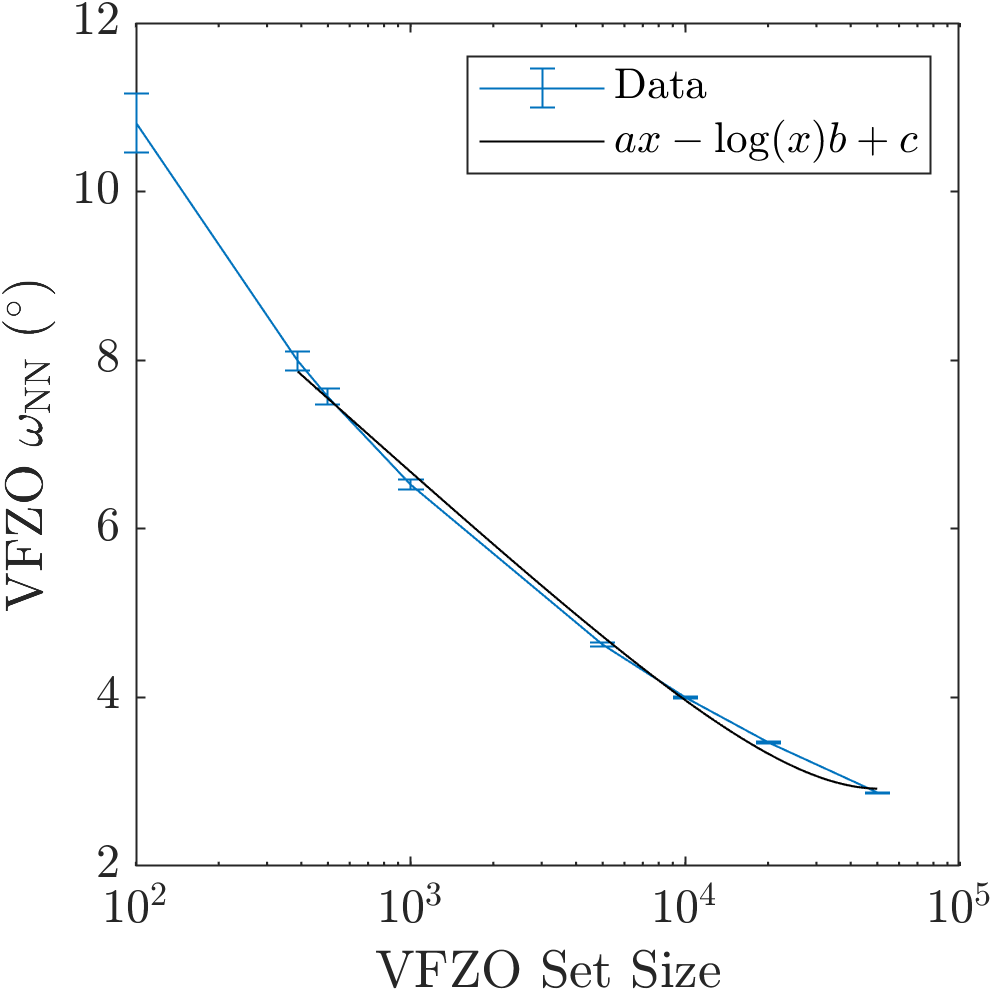
\includegraphics[scale=1]{nndist-vs-setsize.png}
%    \caption{\Gls{nn} \gls{vfzgbo} ($\omega_{\text{NN}}$) distances ($^{\circ}$) versus \gls{vfzgbo} set size out of 70-80 random \gls{vfzgbo} sets per set size and a fit to $ax-\mathrm{log}(x)b+c$ where $a=2.5025\times10^{-5}$, $b=1.27396$, $c=15.4499$, $x$ represents set size, and $388 \leq x \leq 50000$.}
%    \label{fig:nndist-vs-setsize}
%\end{figure}
%
%\Cref{fig:nndist-vs-setsize} illustrates how the \gls{vfzgbo} average \gls{nn} distance varies with the cardinality of the set (i.e. number of random \glspl{vfzgbo} in the set). Additionally, a fitted model is given. For a specific \num{50000} \gls{vfzgbo} set, the \gls{nn} \gls{gbo} distance is \SI{\nnomega{}}{\degree} (\cref{fig:nnhist-knn-50000}a) while the average 100-th \gls{nn} distance is within \SI{10}{\degree} (\cref{fig:nnhist-knn-50000}b). This indicates that, on average, \outpt{} \glspl{vfzgbo} fall within a typical \gls{gb} correlation length (\SI{10}{\degree} \cite{olmstedSurveyComputedGrain2009}) of \inpt{} \glspl{vfzgbo} in large set sizes.
%

\section{Choice of Reference \glsxtrshort{gbo} }
\label{sec:oref}
In \cref{sec:methods:framework:vfz}, we describe how $o_{\text{ref}}$ must be chosen such that it does not coincide with a symmetry operator. In other words, it must be chosen such that symmetry operators do not produce identical coordinates. Randomly generating \glspl{vfzgbo} as in \cref{sec:methods:rand} ensures that with infinite precision, \glspl{gb} will not fall \emph{exactly} on a high-symmetry border. In practice with finite precision and pseudo-random number generation, a \gls{vfzgbo} will rarely be situated (within numerical tolerance) on one of these high-symmetry borders. Indeed, the $o_{\text{ref}}$ typically used in this work is randomly generated\footnote{via \matlab{get_ocubo(1,'random',[],10)}, where \matlab{10} is the random number generator seed. } with \gls{gbo} and \gls{5dof} coordinates given in \cref{tab:oref,tab:oref-qm-nA}, respectively.

The existence of degenerate \glspl{vfzgbo} when performing calculations is checked for within the codebase using tolerance comparisons within \matlab{GBdist4.m}, and warnings of degeneracy are output by \matlab{get_octpairs.m}.

A comparison of distances between  $o_{\text{ref}}$ and each of its symmetric images further reveals that there is a single minimum (0 distance) \gls{seo} (the identity operator), and that the next closest \gls{seo} has a non-negligible distance of \SI{62.8}{\degree} in the original \gls{gbo} sense \cref{fig:oref-seo-dist}. This justifies our usual choice of $o_{\text{ref}}$ as being an appropriate low-symmetry \gls{vfzgbo} to define a \gls{vfz}.

\begin{figure}
    \centering
    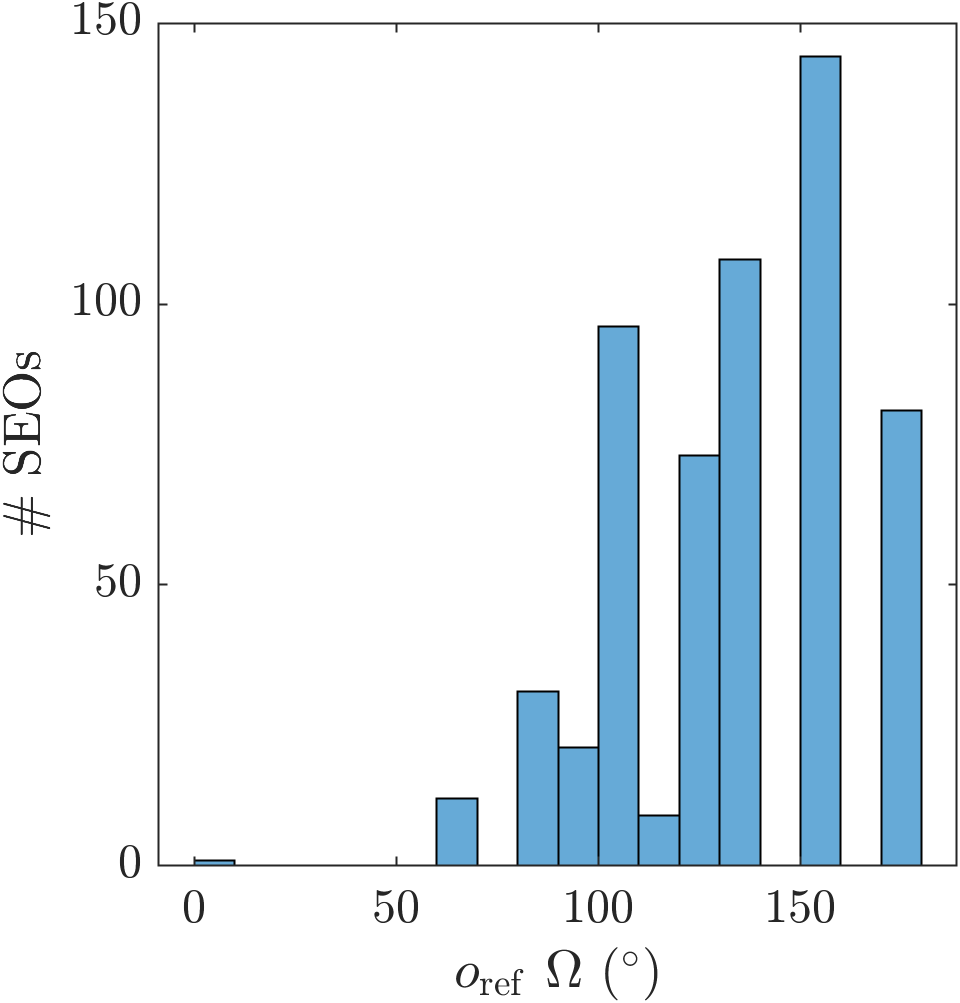
\includegraphics{figures/oref-seo-dist.png}
    \caption{ Histogram of \gls{gbo} distances for all \glspl{seo} for the typical reference octonion ($o_\text{ref}$) used in this work (with coordinates given in \cref{tab:oref}) relative to $o_\text{ref}$. A single minimum distance \gls{seo} (the identity symmetry operator) is found, with a non-negligible next largest distance, justifying this \gls{gb} as an appropriate choice of reference. }
    \label{fig:oref-seo-dist}
\end{figure}

\begin{table}
\centering
\caption{Approximate \gls{gbo} coordinates for a typical $o_\text{ref}$. }
\label{tab:oref}
\begin{tabular}{@{}llllllll@{}}
\toprule
o(1)   & o(2)    & o(3)    & o(4)   & o(5)   & o(6)   & o(7)    & o(8)   \\ \midrule
0.7319 & -0.6330 & -0.2523 & 0.0025 & 0.0939 & 0.8641 & -0.3277 & 0.3704
\end{tabular}
\end{table}

\begin{table}
\centering
\caption{Approximate misorientation quaternion (qm) and boundary plane normal (nA) coordinates for a typical $o_\text{ref}$. }
\label{tab:oref-qm-nA}
\begin{tabular}{@{}lllllll@{}}
\toprule
qm(1)   & qm(2)  & qm(3)   & qm(4)   & nA(1)  & nA(2)   & nA(3)  \\ \midrule
-0.3946 & 0.7845 & -0.4527 & -0.1546 & 0.3661 & -0.9278 & 0.0713
\end{tabular}
\end{table}

\section{Euclidean and Arc Length Distances}
\label{sec:supp:dist-parity}

In addition to enabling us to leverage the machinery of efficient and established algorithms, the choice of using Euclidean distance as opposed to hyperspherical arclength can be justified by the following observations:
\begin{itemize}
	\item The minimum Euclidean distance \gls{seo} will be the same as the minimum arc length distance \gls{seo} because $d_{\text{S}}$ is a monotonically increasing function of $d_{\text{E}}$, for $d_{\text{S}}\!\left(d_{\text{E}}\right)\in[0,\pi]$ (\cref{fig:dist-parity}). 
	\item For the FCC point group symmetry ($m\bar{3}m$) the portion of $\mathbb{S}^7$ subtended by the \gls{vfz} is sufficiently small that the approximation $d_{\text{E}} \simeq d_{\text{S}}$ holds to very high accuracy\footnote{This is true for a specific pair of \glspl{gbo} within a \gls{vfz}. When calculating the \emph{minimum} distance between \glspl{seo} of two points, there are additional considerations that must be attended to as discussed in detail in \cref{sec:methods:framework:vfz-dist}.} as shown in \cref{fig:dist-parity}. 
	\item Calculation of $d_{\text{E}}$ does not require the use of any inverse trigonometric functions and is about \SI{23}{\percent} faster than calculation of $d_{\text{S}}$ or $d_\Omega$.
\end{itemize}

The close correlation between Euclidean and arc length distances in the \gls{vfzgbo} sense is shown in \cref{fig:dist-parity} using pairwise distances of \num{10000} \glspl{vfzgbo}. This justifies our use of Euclidean distance as an approximation of hyperspherical arc length (and by extension, that a scaled Euclidean distance approximates a non-symmetrized \gls{gbo} distance, see \cref{eq:8Deuclidean_dist,eq:7sphere_arc_length,eq:omega} of the main paper). However, comparison with the original \gls{gbo} metric \cite{francisGeodesicOctonionMetric2019} gives overestimation for some boundaries. This is an inherent feature of the \gls{vfz} framework that can be addressed via use of the ensemble methods described in \cref{sec:methods:framework:vfz-dist} (see also \cref{fig:dist-ensemble-k1-2-10-20,fig:dist-ensemble-rmse-mae}).

\begin{figure}
\centering
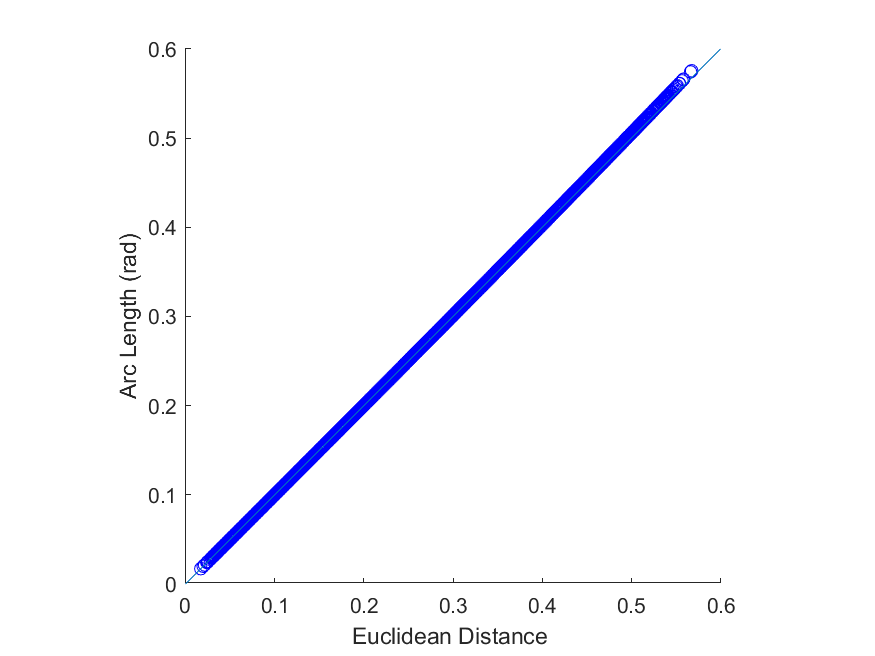
\includegraphics[scale=1]{dist-parity.png}
\caption{Parity plot of 8D Cartesian hyperspherical arc length vs. 8D Cartesian Euclidean distance for pairwise distances in a ($m\bar{3}m$) symmetrized set of \num{10000} randomly sampled \glspl{vfzgbo}. The max arc length is approximately \SI{0.58}{\radian}, indicating a max \gls{gbo} distance of approximately \SI{1.16}{\radian} or \SI{66.5}{\degree} between any two points in the \gls{vfz}. The close correlation between arc length and Euclidean distance supports the validity of using Euclidean distance instead of arc length in the interpolation methods. This is \textit{separate} from the correlation between \gls{vfzgbo} Euclidean or arc length distances with the traditional \gls{gbo} distance \cite{chesserLearningGrainBoundary2020}.}
\label{fig:dist-parity}
\end{figure}

Additionally, the use of an isometry equivalence relationship in \citet{morawiecDistancesGrainInterfaces2019} in a non-\gls{vfz} sense results in identical distance results within numerical tolerance (\cref{fig:pd-fix}).

\begin{figure}
    \centering
    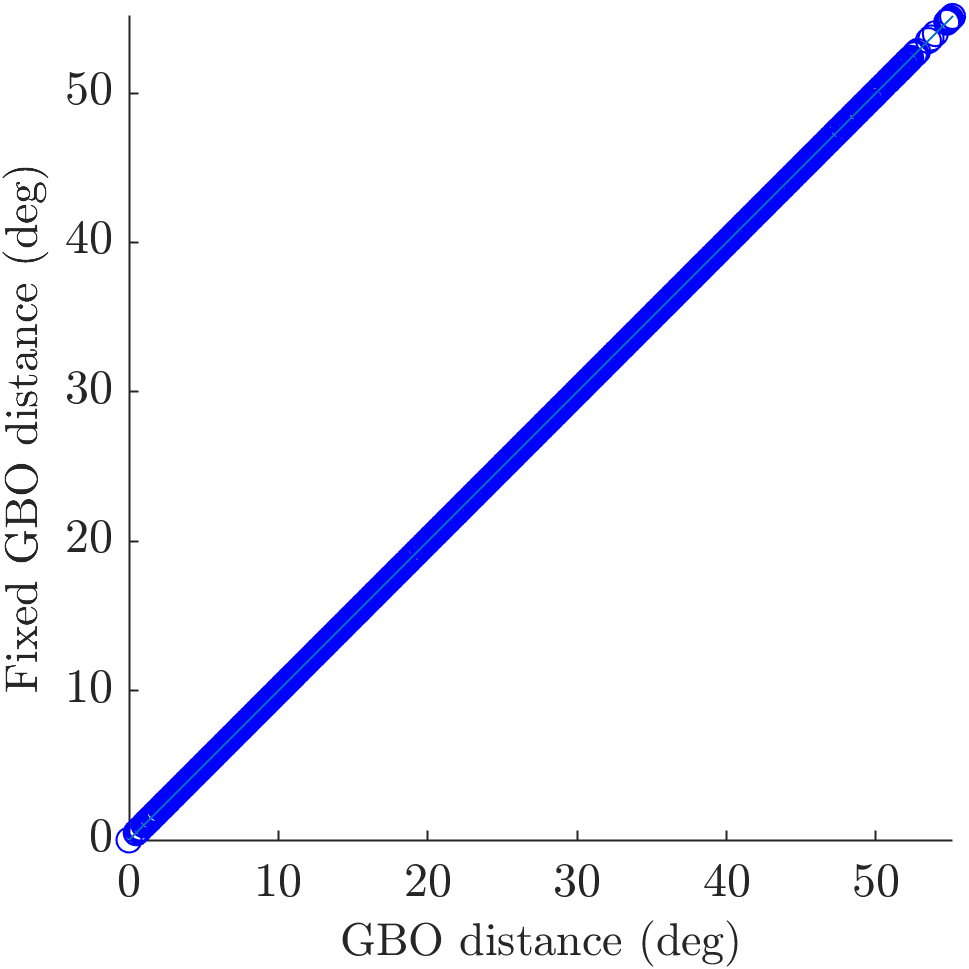
\includegraphics{figures/pd-fix.png}
    \caption{\Gls{gb} distances calculated with one \gls{gbo} fixed vs. the traditional calculations in \citet{chesserLearningGrainBoundary2020} show that the isometry equivalence discussed in \citet{morawiecDistancesGrainInterfaces2019} applies to \glspl{gbo}. The pairwise-distance matrix for the Olmsted \glspl{gb} supplied in \cite{chesserGBOctonionCode2019} was used. }
    \label{fig:pd-fix}
\end{figure}

\section{Computational Complexity of \glsentryshort{vfz} vs. \glsentryshort{gbo} Distances } \label{sec:computational-complexity}
Let $o_1$ and $o_2$ denote two \glspl{gb} represented in \gls{gbo} coordinates. 
To perform a traditional symmetrized \gls{gbo} distance calculation according to \citet{francisGeodesicOctonionMetric2019}, we compare all \glspl{seo} of $o_1$ to all of the \glspl{seo} of $o_2$ and take the smallest distance. If $N_p$ is the number of proper rotations of the crystallographic point group, this single minimum distance calculation requires a total of $4N_p^4$ \glspl{seo} to be considered (Sections 4.3 and 4.5 of \citet{francisGeodesicOctonionMetric2019}). Thus, the total number of \gls{seo} computations will be $4N_p^4L^2$. However, it is possible to fix a single \gls{gb} in the \gls{gb} pair and still obtain accurate\footnote{Compared with the pairwise distance matrix of the 388 Olmsted \glspl{gb}, we obtained a \gls{rmse} of \SI{1.6566E-7}{\degree} for this computation which completed in \SI{133}{\s} using 6 cores (see \matlab{get_pd_fix.m})} due to isometry equivalence (see Section 7 of \cite{morawiecDistancesGrainInterfaces2019} and \cref{fig:pd-fix}).

In contrast, for a single distance calculation using the \gls{vfz} framework, $o_1$ and $o_2$ are first mapped into the \gls{vfz}, and then only a single distance calculation is required between them. Mapping $o_1$ into the \gls{vfz} requires comparison of $8N_p^2$ \glspl{seo}\footnote{This is 8 instead of 4 because the simplifying assumption that only two of the four double cover cases need to be considered \cite{francisGeodesicOctonionMetric2019} does not apply in the \gls{vfz} framework. This is confirmed by applying \matlab{uniquetol()} on a set of $4608$ \glspl{gbo} which has a final set size of $4608$, where $4608=8\times N_p^2$ and $N_p=24$ (see \matlab{osymset.m}).} of $o_1$ with a fixed reference \gls{gb} in the interior of the \gls{vfz}; and likewise for $o_2$. Consequently, a single distance calculation between $o_1$ and $o_2$ under the \gls{vfz} framework requires $O(N_p^2)$ \gls{seo} computations. If one desires to compute a pairwise distance matrix between $L$ \glspl{gb}, the total computational cost\footnote{See \cref{sec:results:efficiency:symruntime} for a detailed explanation of why this is \emph{not} $O(N_p^2L^2)$.} will be $O(N_p^2L)$, which represents a dramatic reduction compared to the traditional approach.

\section{Additional Interpolation Results}

\subsection{Smaller Set Sizes of Input GBs}
Interpolation results for \num{388} and \num{10000} \glspl{gb} are given in \cref{fig:brkparity388} and \cref{fig:brkparity10000}, respectively.

\begin{figure}[!ht]
    \centering
    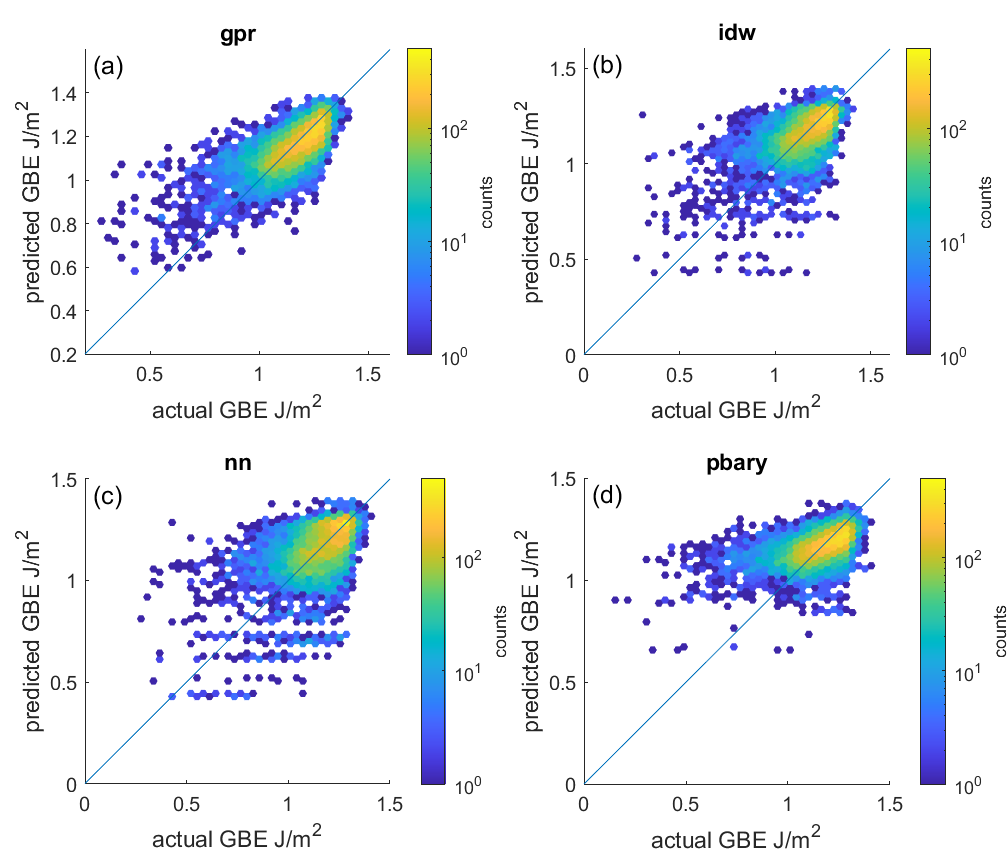
\includegraphics[scale=1]{brkparity388.png}
    \caption{Hexagonally binned parity plots for \num{388} \inpt{} and \num{10000} \outpt{} \glspl{gbo} formed via pairs of a random cubochorically sampled quaternion and a spherically sampled random boundary plane normal. Interpolation via (a) \gls{gpr}, (b) \gls{idw}, (c) \gls{nn}, and (d) barycentric coordinates.  \gls{brk} \gls{gbe} function for \gls{fcc} Ni \cite{bulatovGrainBoundaryEnergy2014} was used as the test function.}
    \label{fig:brkparity388}
\end{figure}

\begin{figure}[!ht]
    \centering
    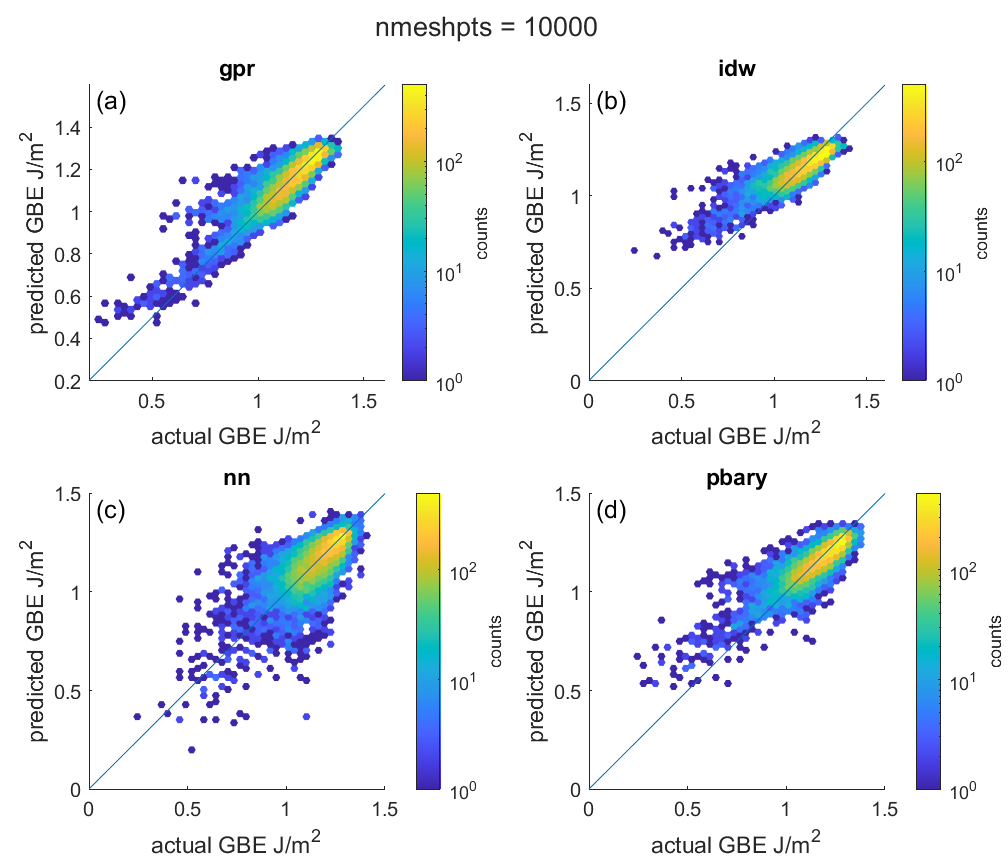
\includegraphics[scale=1]{brkparity10000.png}
    \caption{Hexagonally binned parity plots for \num{10000} \inpt{} and \num{10000} \outpt{} \glspl{gbo} formed via pairs of a random cubochorically sampled quaternion and a spherically sampled random boundary plane normal. Interpolation via (a) \gls{gpr}, (b) \gls{idw}, (c) \gls{nn}, and (d) barycentric coordinates.  \gls{brk} \gls{gbe} function for \gls{fcc} Ni \cite{bulatovGrainBoundaryEnergy2014} was used as the test function.}
    \label{fig:brkparity10000}
\end{figure}

\subsection{Octonions used for 1D Arcs}
The octonions used in \cref{fig:tunnel-50000,fig:kim-interp} are given in \cref{tab:tunnel-AB,tab:tunnel-AB2}, respectively. The misorientation quaternions and \gls{bp} normal pairs are likewise given in \cref{tab:tunnel-AB-qm-nA,tab:tunnel-AB2-qm-nA}, respectively. Disorientations are likewise plotted in Rodrigues space (see \cite{patalaSymmetriesRepresentationGrain2013})\footnote{Note that octonions A and B in this work have no correspondence with points A and B described in \cite{patalaSymmetriesRepresentationGrain2013}. } in \cref{fig:ABrod,fig:ABrod-kim}, respectively. Conversion of \gls{bp} normals that maintains consistency during conversion from misorientation to disorientation has not been implemented; therefore, visualizations of \gls{bp} normal are not provided and \gls{bp} normal is only reported alongside its misorientation as $qm$/$nA$ pairs.
% Please add the following required packages to your document preamble:
% \usepackage{booktabs}
\begin{table*}[]
\centering
\caption{Approximate coordinates of \glspl{vfzgbo} A and B used for the interpolation in \cref{fig:tunnel-50000}. Individual quaternions of each \gls{gbo} are given in the laboratory reference frame with an assumed \gls{gb} normal pointing in the +z direction, also in the laboratory reference frame.}
\label{tab:tunnel-AB}
\begin{tabular}{@{}lllllllll@{}}
\toprule
Octonion & o(1)   & o(2)    & o(3)    & o(4)    & o(5)    & o(6)   & o(7)    & o(8)   \\ \midrule
A        & 0.3419 & -0.5466 & -0.2657 & -0.1174 & -0.1000 & 0.5871 & -0.2329 & 0.3018 \\
B        & 0.6275 & -0.2817 & -0.1167 & 0.1154 & 0.2322 & 0.5891 & -0.2446 & 0.1979 \\ \bottomrule
\end{tabular}
\end{table*}

\begin{table*}[]
\centering
\caption{Approximate misorientation quaternion (qm) and boundary plane normal (nA) coordinates of \glspl{vfzgbo} A and B for the interpolation in \cref{fig:tunnel-50000}. }
\label{tab:tunnel-AB-qm-nA}
\begin{tabular}{@{}llllllll@{}}
\toprule
Octonion & qm(1) & qm(2) & qm(3) & qm(4) & nA(1) & nA(2) & nA(3) \\ \midrule
A & -0.6573 & 0.5072 & -0.4044 & -0.3836 & 0.6200 & -0.6227 & -0.4774 \\
B & 0.0622 & 0.8599 & -0.5002 & -0.0805 & 0.1628 & -0.7609 & 0.6281 \\ \bottomrule
\end{tabular}
\end{table*}

\begin{figure}
    \centering
    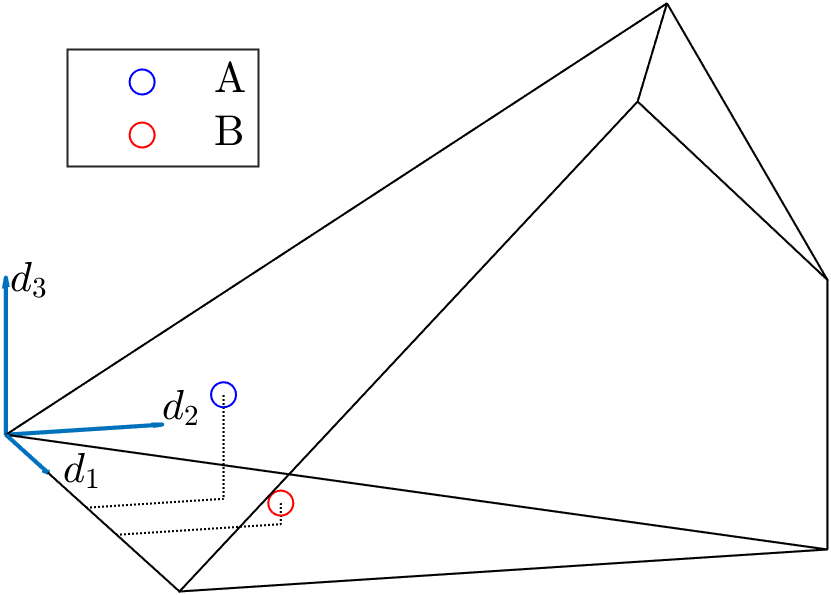
\includegraphics{figures/ABrod.png}
    \caption{Disorientations for octonions A and B (from \cref{fig:tunnel-50000}) plotted in Rodrigues space. }
    \label{fig:ABrod}
\end{figure}

\begin{table*}
\centering
\caption{Approximate coordinates of \glspl{vfzgbo} $A$ and $B$ used for the \gls{ms} Fe simulation dataset interpolation in \cref{fig:kim-interp}. Individual quaternions of each \gls{gbo} are given in the laboratory reference frame with an assumed \gls{gb} normal pointing in the +z direction, also in the laboratory reference frame.}
\label{tab:tunnel-AB2}
\begin{tabular}{lllllllll}
\hline
Octonion & o(1)   & o(2)    & o(3)    & o(4)    & o(5)    & o(6)   & o(7)    & o(8)   \\ \hline
A        & 0.6163 & -0.2916 & -0.1313 & 0.1338 & 0.2225 & 0.5911 & -0.2697 & 0.1684 \\
B        & 0.3105 & -0.5555 & -0.2929 & -0.0961 & -0.0973 & 0.5715 & -0.2620 & 0.3087 \\ \hline
\end{tabular}
\end{table*}

\begin{table*}[]
\centering
\caption{Approximate misorientation quaternion (qm) and boundary plane normal (nA) coordinates of \glspl{vfzgbo} A and B for the \gls{ms} Fe simulation dataset interpolation in \cref{fig:kim-interp}. }
\label{tab:tunnel-AB2-qm-nA}
\begin{tabular}{@{}llllllll@{}}
\toprule
Octonion & qm(1) & qm(2) & qm(3) & qm(4) & nA(1) & nA(2) & nA(3) \\ \midrule
A & 0.0454 & 0.8303 & -0.5305 & -0.1645 & 0.1676 & -0.7891 & 0.5909 \\
B & -0.6012 & 0.4780 & -0.4528 & -0.4528 & 0.5774 & -0.5774 & -0.5774 \\ \bottomrule
\end{tabular}
\end{table*}

\begin{figure}
    \centering
    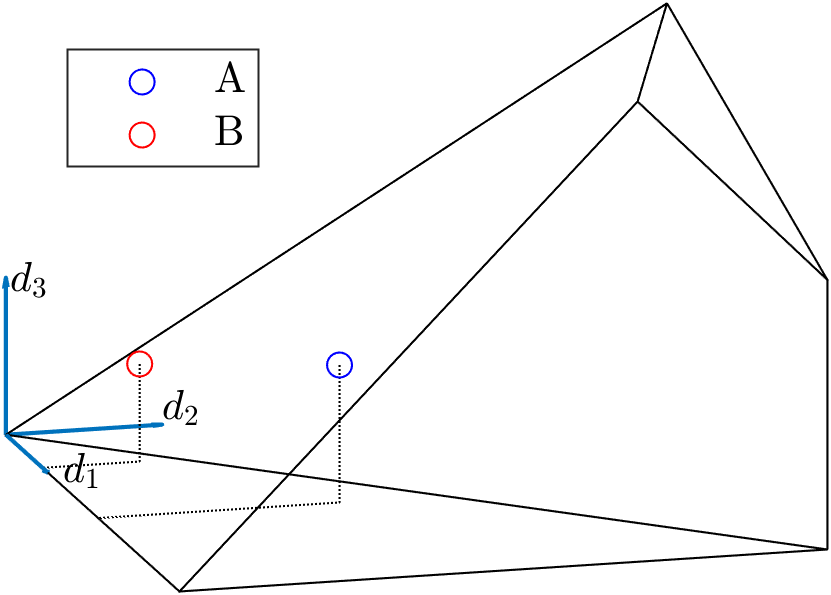
\includegraphics{figures/ABrod-kim.png}
    \caption{Disorientations for octonions A and B (\gls{ms} Fe simulation dataset interpolation in \cref{fig:kim-interp}) plotted in Rodrigues space. }
    \label{fig:ABrod-kim}
\end{figure}

%
%The corresponding \gls{5dof} coordinates are:
\section{Mitigating Distance Overestimation} \label{sec:overestimation}
Overestimation imposes a "sparseness" of data within a local region of influence common to the interpolation methods in this work, whereas underestimation would give erroneous high correlations between uncorrelated \glspl{gb}. Because only overestimation relative to traditional \gls{gbo} distances exist in this work (as shown in \cref{fig:dist-ensemble-k1-2-10-20}), we expect that large errors will occur infrequently (\cref{sec:results:accuracy}). 

While distance calculations are subject to these infrequent overestimates, they are largely immaterial for interpolation. This is because all interpolation methods in this work involve a region of influence that is small when the point set size is large, so that if the distance to a \gls{nn} is overestimated it simply does not contribute to the interpolation (the "sparseness" referred to earlier). Consequently the accuracy of the interpolation is not significantly impacted by infrequent distance overestimates, and excellent results can be achieved without addressing this limitation. However, if even greater accuracy is desired it can be obtained for a relatively minor cost by considering multiple \glspl{vfz}.

We find that taking the minimum distance among several \gls{vfzgbo} sets defined by separate reference \glspl{gbo} leads to better correlation between the Euclidean approximation and the traditional \gls{gbo} metric as shown in \cref{fig:dist-ensemble-k1-2-10-20}. Additionally, \cref{fig:dist-ensemble-rmse-mae} shows that the error between scaled Euclidean distance and the traditional \gls{gbo} metric decreases rapidly as the number of ensemble \gls{vfzgbo} components increases. This confirms that employing a small ensemble of \gls{vfzgbo} sets results in significant improvement to the Euclidean distance approximation (\cref{fig:dist-ensemble-k1-2-10-20,fig:dist-ensemble-rmse-mae}) of the traditional \gls{gbo} metric. However, as already mentioned, improvements to interpolation results are expected to be less significant since they are already robust to occasional distance overestimates. In terms of computational runtime, use of an ensemble of 10 \glspl{vfz} will increase runtime by a factor of $\sim$10 via a loop-based implementation. For a symmetrized $\num{50000}\times\num{50000}$ pairwise distance matrix, this results in a runtime of approximately 1~CPU~hour instead of $\sim$7~CPU~minutes for a single \gls{vfz}. However, this is still much faster than the original \gls{gbo} approach used in \cite{chesserLearningGrainBoundary2020}, which would take an estimated 6.6 CPU years using the original implementation (or 153 CPU days if one \gls{gb} in the \gls{gb} pair is fixed according to the assumption in \citet{morawiecDistancesGrainInterfaces2019}). Additionally, it may be worthwhile to make the distance calculations GPU-compatible for further speed-up. %might be worth making a note here about how many function calls you might expect during a single grain growth simulation. Then we can translate these times into expected minimum CPU time for a 3D grain growth simulation for X number of grains. Maybe Jose has an estimate for this. I think I included something later

\section{Ensemble Interpolation Results}
\label{sec:ensemble-interp}
Ensemble interpolation is a classic technique that can be used to enhance predictive performance of models. Here we describe our methods (\cref{sec:ensemble-interp:methods}), results (\cref{sec:ensemble-interp:results}), and the potential of integrating ensemble interpolation with a \gls{gprm} scheme (\cref{sec:ensemble-interp:egprm}).

\subsection{Methods}
\label{sec:ensemble-interp:methods}
\Gls{vfzgbo} ensemble\footnote{Ours is a "bagging"-esque ensemble scheme because the same interpolation method (\glsxtrshort{gpr}) is used but with different representations for the \inpt{} data. } interpolation occurs by:
\begin{enumerate}
    \item generating multiple reference \glspl{gbo} to define multiple \glspl{vfz}
    \item obtaining multiple \gls{vfzgbo} representations for a set of \glspl{gb} based on the various reference \glspl{gbo}
    \item performing an interpolation (e.g. \gls{gpr}) for each of the representations
    \item homogenizing the ensemble of models (e.g. by taking the mean or median of the various models)
\end{enumerate}

\subsection{Results}
\label{sec:ensemble-interp:results}

Use of an ensemble interpolation scheme decreases interpolation error for a \gls{gpr} model with \num{50000} \inpt{} and \num{10000} \outpt{} \glspl{vfzgbo}. By using an ensemble size of 10 (i.e. 10 \gls{gpr} models each with different reference \glspl{gbo} and therefore different \glspl{vfz}), \gls{rmse} and \gls{mae} decreased from \SIlist{0.0241;0.0160}{\J\per\square\m} to \SIlist{0.0187;0.0116}{\J\per\square\m}, respectively, using the median homogenization function (\cref{fig:ensemble-interp-rmse-mae}). 
\begin{figure}
    \centering
    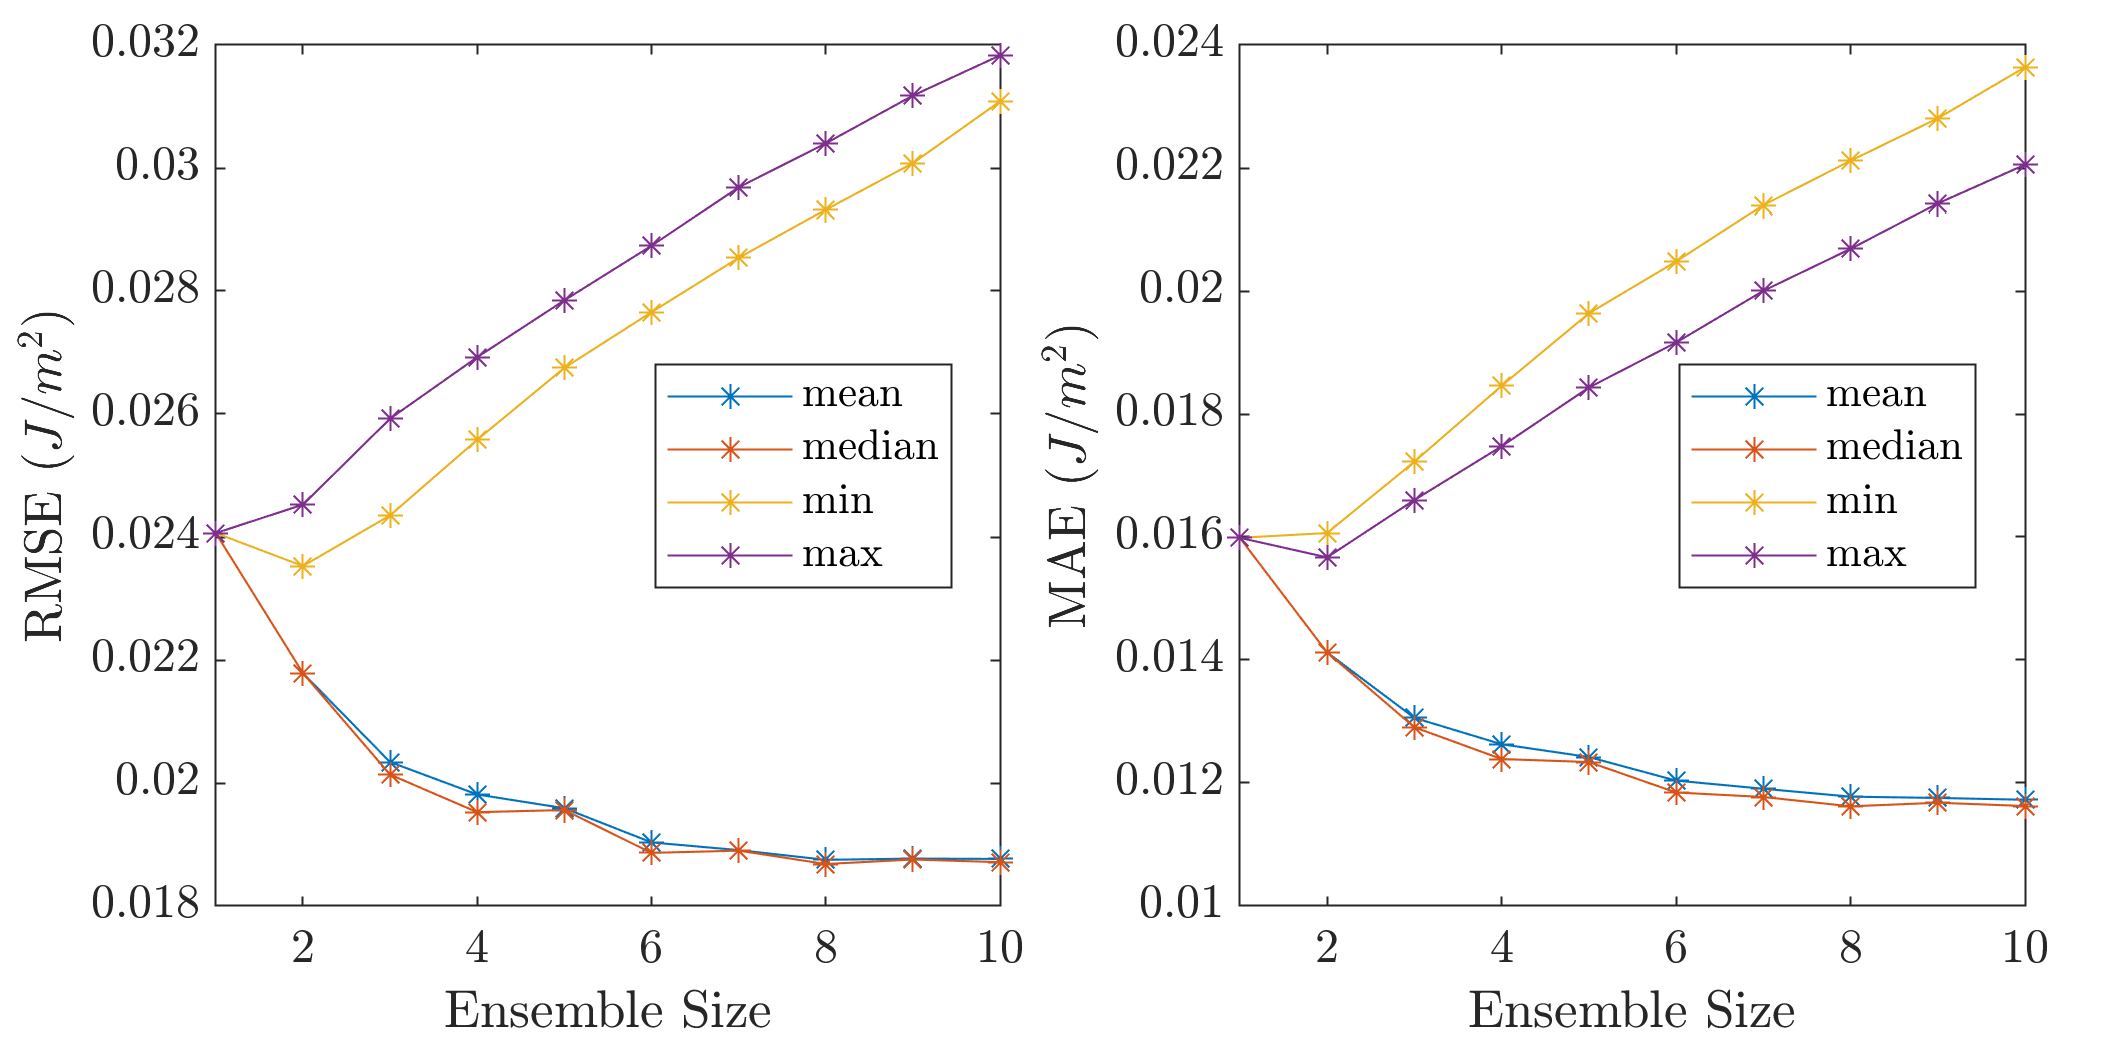
\includegraphics[scale=1]{figures/ensemble-interp-rmse-mae.png}
    \caption{(a) \Gls{rmse} and (b) \gls{mae} vs. ensemble size for mean, median, minimum, and maximum homogenization functions. A \gls{gpr} model with \num{50000} \inpt{} and \num{10000} \outpt{} \glspl{vfzgbo} was used. }
    \label{fig:ensemble-interp-rmse-mae}
\end{figure}

\Cref{fig:ensemble-interp} shows the hexagonally binned parity plots for predictions made using the mean, median, minimum, and maximum predicted values over an ensemble of 10 \glspl{vfz}. Qualitatively, the ensemble mean and ensemble median parity plots look similar to those from the main text (\cref{fig:brkparity50000}), though the distributions of the ensemble scheme are somewhat tighter. The ensemble minimum produces better predictions of low \gls{gbe} than any of the other models, but underestimates high \gls{gbe} as expected. Naturally, the ensemble maximum overestimates in general. Diminishing returns manifest in \cref{fig:ensemble-interp-rmse-mae} for mean and median homogenizations. This is to be expected because the original \gls{gbo} distances \cite{francisGeodesicOctonionMetric2019} are well-approximated using an ensemble size of 10 (\cref{fig:dist-ensemble-k1-2-10-20}c and \cref{fig:dist-ensemble-rmse-mae}).
\begin{figure}[h!]
    \centering
    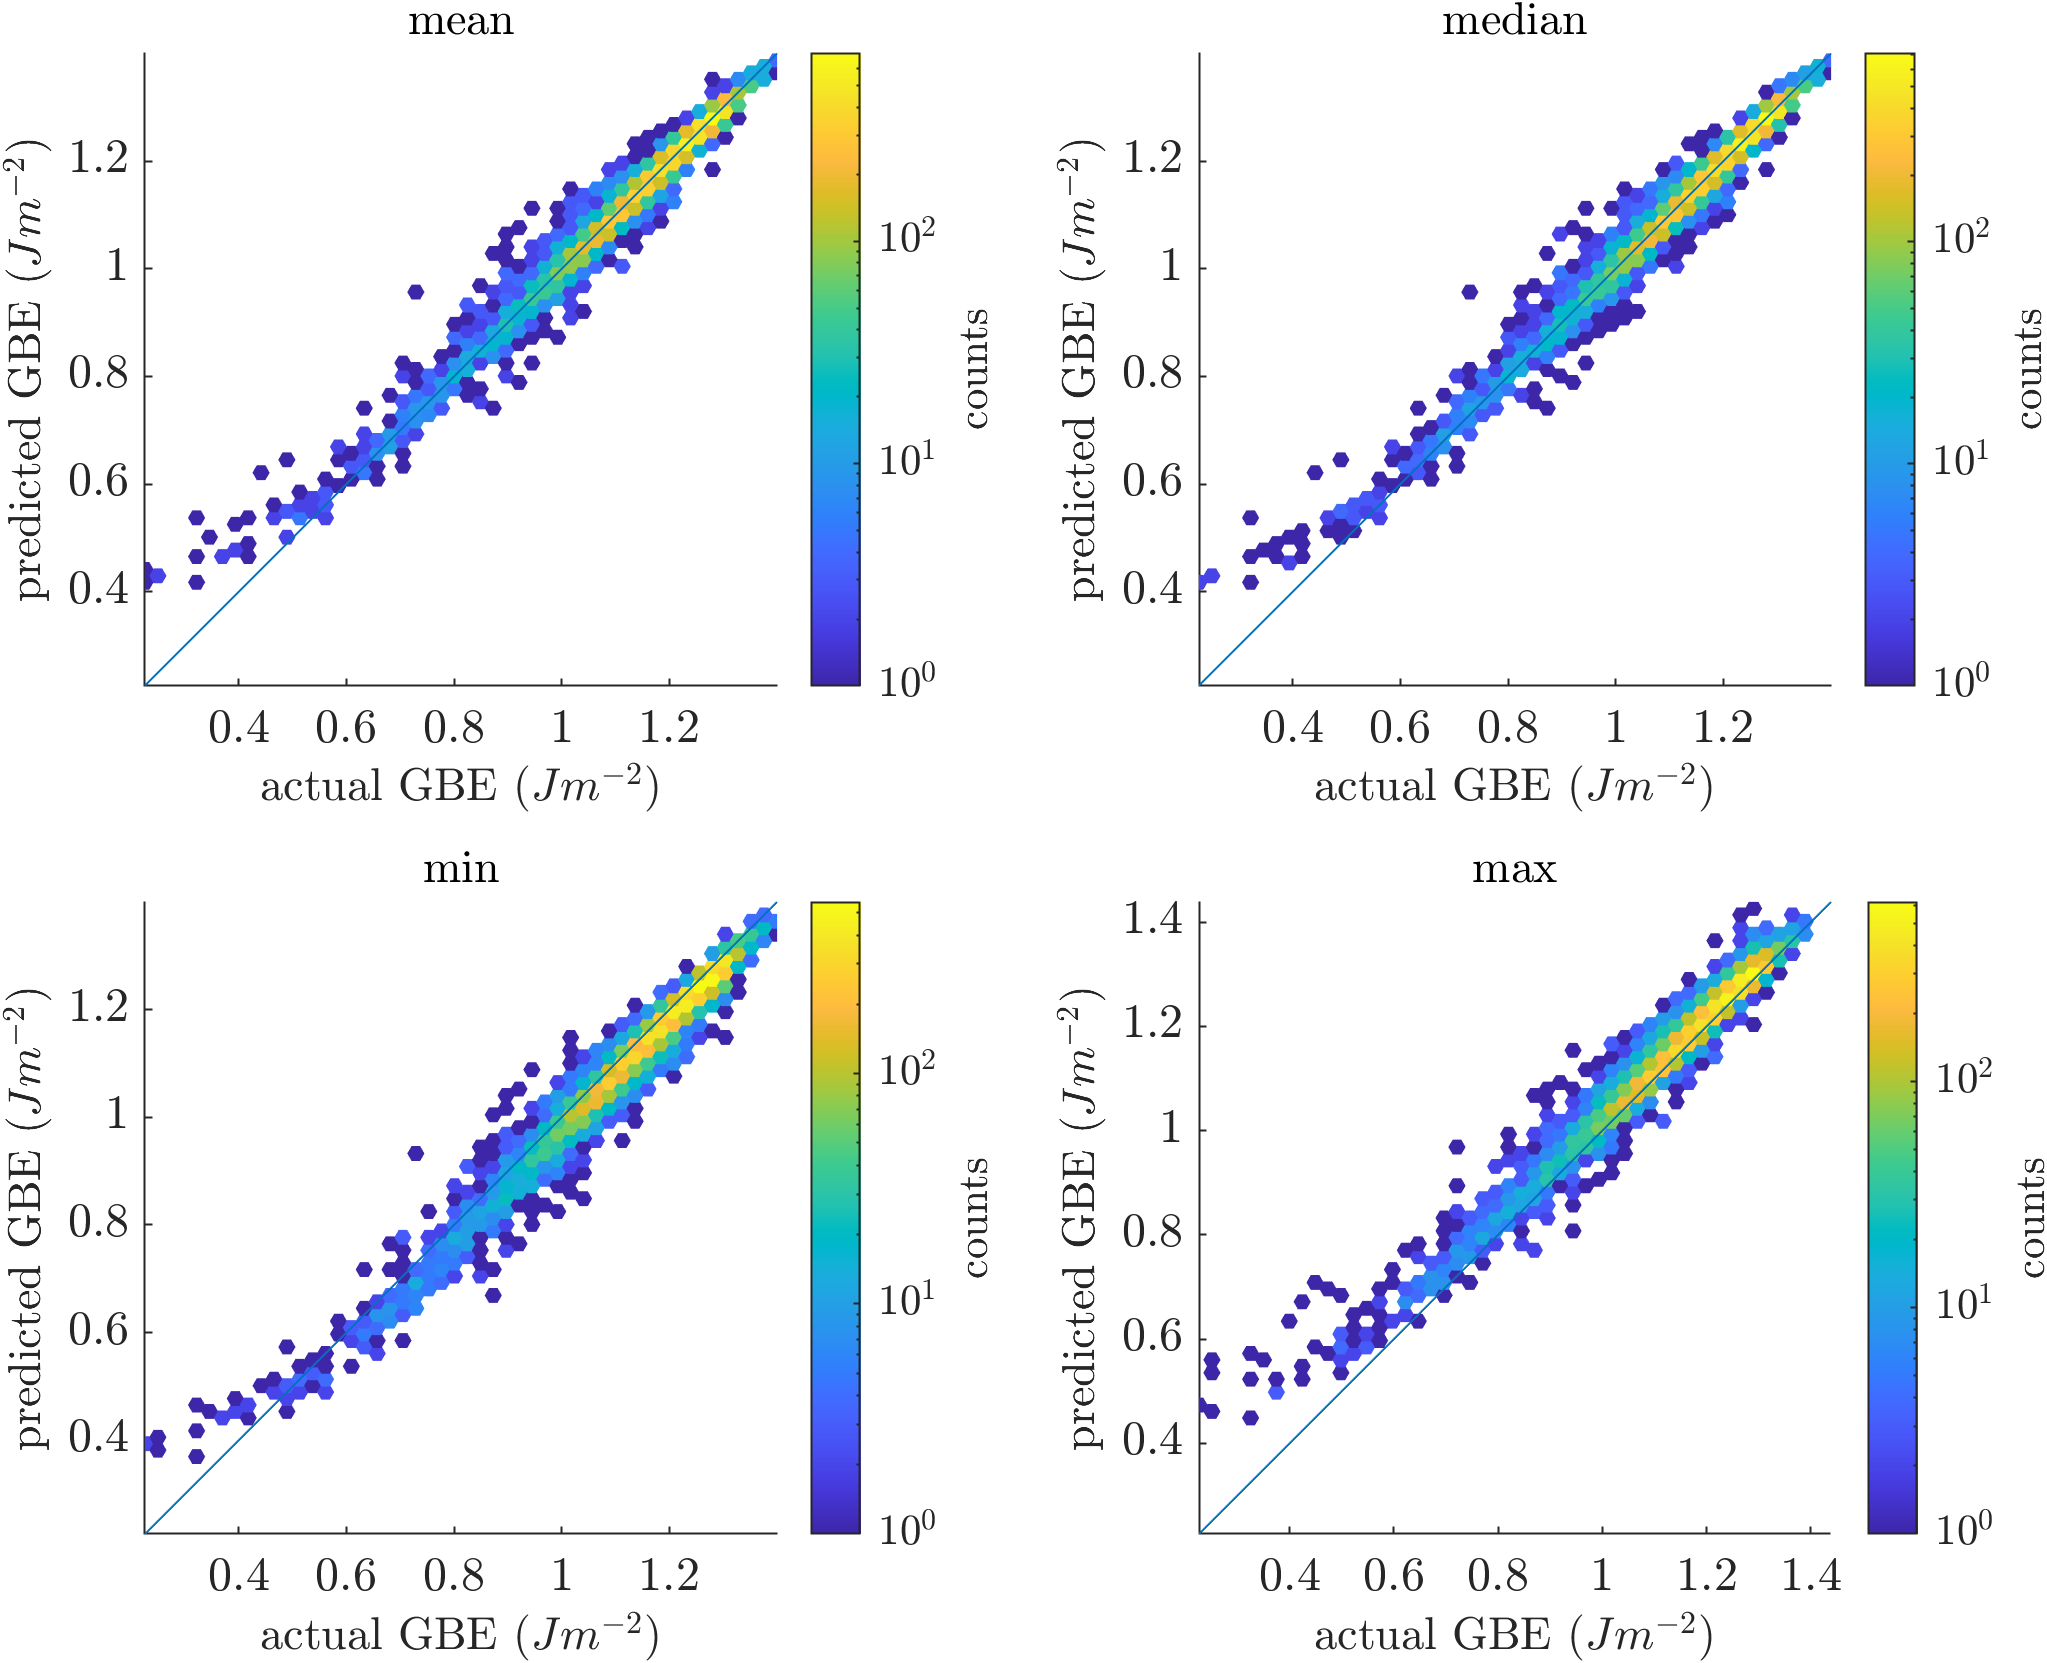
\includegraphics[scale=1]{figures/ensemble-interp.png}
    \caption{Hexagonally binned parity plots for (a) mean, (b) median, (c) minimum, and (d) maximum ensemble homogenization functions. A \gls{gpr} model with \num{50000} \inpt{} and \num{10000} \outpt{} \glspl{vfzgbo} was used. }
    \label{fig:ensemble-interp}
\end{figure}

\subsection{Possibility: Combining Ensemble with \glsentrytitlecase{gpr}{long} Mixture}
\label{sec:ensemble-interp:egprm}

A scheme which preferentially favors the ensemble minimum for low \gls{gbe} predictions and defaults to ensemble mean or median for all other \glspl{gbe} may produce even better results across the full range of \glspl{gbe}. For example, this could be accomplished by combining the ensemble scheme described here with the \gls{gpr} mixture model described in \cref{sec:supp:kim-interp:method}.
%
% \section{Barycentric Interpolation}
% \label{sec:supp:bary}
%
% \subsection{High-Aspect Ratios}
% \label{sec:supp:bary:artifact}
% An artifact of the barycentric interpolation method which occurs due to the presence of high-aspect ratio facets is shown in \cref{fig:high-aspect-non-int}. As the dimensionality increases for a constant number of points and from our numerical tests, the rate of missed facet intersections increases. This artifact and our method for addressing it are discussed in \cref{sec:app:bary:int} of the main text.

% \begin{figure*}
%     \centering
%     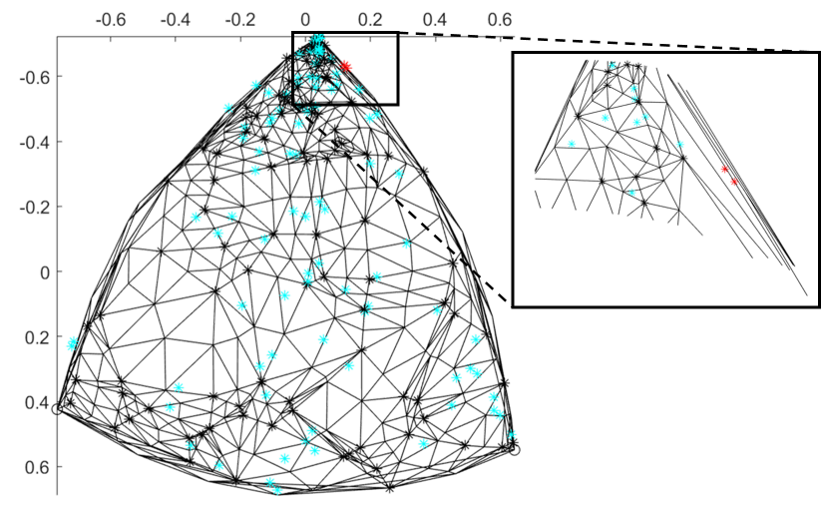
\includegraphics[scale=1]{figures/high-aspect-non-int.png}
%     \caption{Illustration of two \outpt{} points (red) for which no intersecting facet is found due to being positioned within a high-aspect ratio facet. The inset shows that facets connected to the \gls{nn} do not contain the \outpt{} point. Many \glspl{nn} would need to be considered before an intersection is found. Additionally, it is expected that if found, the interpolation will suffer from higher error due to use of facet vertices far from the interpolation point. Proper intersections of \outpt{} points with the mesh are shown in blue.}
%     \label{fig:high-aspect-non-int}
% \end{figure*}

% \subsection{Use of Alternative Distance Metrics}
%

\section{Literature Datasets}

\subsection{\glsentrytitlecase{gpr}{long} for Fe Simulation Dataset} % move these to supp?
\label{sec:methods:gprsim}
The Fe simulation data is obtained from \cite{kimPhasefieldModeling3D2014} rather than \cite{kimIdentificationSchemeGrain2011} due to a mistake in the earlier dataset file\footnote{We were informed of the error during an email discussion with the corresponding author of \cite{kimPhasefieldModeling3D2014}.}. \Glspl{gb} with a \gls{gbe} less than \SI{0.01}{\joule\per\square\meter} are removed to get rid of "no-boundary" \glspl{gb}. Repeated \glspl{gb} are then identified and removed by converting all \glspl{gb} into a \gls{vfzgbo} set (see \matlab{Kim2oct.m}) and sorting the repeated \glspl{gb} into "degenerate sets"\footnote{A degenerate "set" is distinct from a \glspl{vfzgbo} "set". This sorting occurs via \matlab{avgrepeats.m} with \matlab{avgfn='min'}.}, and only the average \gls{gbe} (and a single \gls{gb}) within each degenerate set was retained. %We estimate the intrinsic \gls{rmse} and \gls{mae} of the Fe simulation dataset to be \SIlist{0.06529;0.06190}{\joule\per\square\meter}, respectively. Minimum and maximum error was \SIlist{-0.2625;0.2625}{\joule\per\square\meter}, respectively. See \cref{sec:supp:kim-interp:quality} for further details on methods used to estimate intrinsic error of the Fe simulation dataset.

\subsection{\glsentrytitlecase{gpr}{long} for Ni Simulation Dataset}
\label{sec:methods:gprsim-Ni}

We use the \gls{gbo} representations\footnote{Contained in \matlab{'olm_octonion_list.txt'} from \citet{chesserGBOctonionCode2019}. } \cite{chesserLearningGrainBoundary2020} of \glspl{gb} from \cite{olmstedSurveyComputedGrain2009}, importing and converting them to the convention used in this work (\cref{sec:app:convention} by taking the quaternion inverse of each of the \glspl{gbo}' quaternions. We take \gls{gbe} values\footnote{Contained in first column of \matlab{'olm_properties.txt'} from  \citet{chesserGBOctonionCode2019}. }, and use a \gls{gpr} model (\cref{sec:methods:interp:gpr}).

\subsection{\glsentrytitlecase{gprm}{long} for Fe Simulation Dataset}
\label{sec:methods:gprmix}
Separate from the four main methods analyzed in this work, a \gls{gprm} model is developed to better predict low \gls{gbe} using the non-uniformly distributed, noisy, Fe simulation dataset described in \cref{sec:methods:gprsim}. An exponential rather than a squared exponential kernel was used for the subset \gls{gpr} model (\cref{sec:supp:kim-interp:method}) to accommodate sharper transitions to better approximate low \glspl{gbe}.

\subsection{Details of \glsentrytitlecase{gpr}{long} Mixture}
\label{sec:supp:kim-interp:method}

A \gls{gpr} mixing model is developed to accommodate the non-uniformly distributed, noisy Fe simulation data \cite{kimPhasefieldModeling3D2014} and better predict low \gls{gbe}. The code implementation is given in \texttt{gprmix.m} and \texttt{gprmix\_test.m} of the \vfzorepo{} \cite{bairdFiveDegreeofFreedom5DOF2020}.

As shown in \cref{fig:kim-interp-teach}a, prediction using the standard approach of the main document (termed the $\epsilon_1$ model) overestimates low \glspl{gbe} for this dataset. By training the model on only \glspl{gb} with a \gls{gbe} less than \thrtwo{} (termed the $\epsilon_2$ model) and by using an exponential (\matlab{KernelFunction='exponential'}) rather than a squared exponential kernel, prediction of low \glspl{gbe} improves, but naturally underestimation occurs for higher \glspl{gbe} (\cref{fig:kim-interp-teach}b).

\begin{figure}
    \centering
    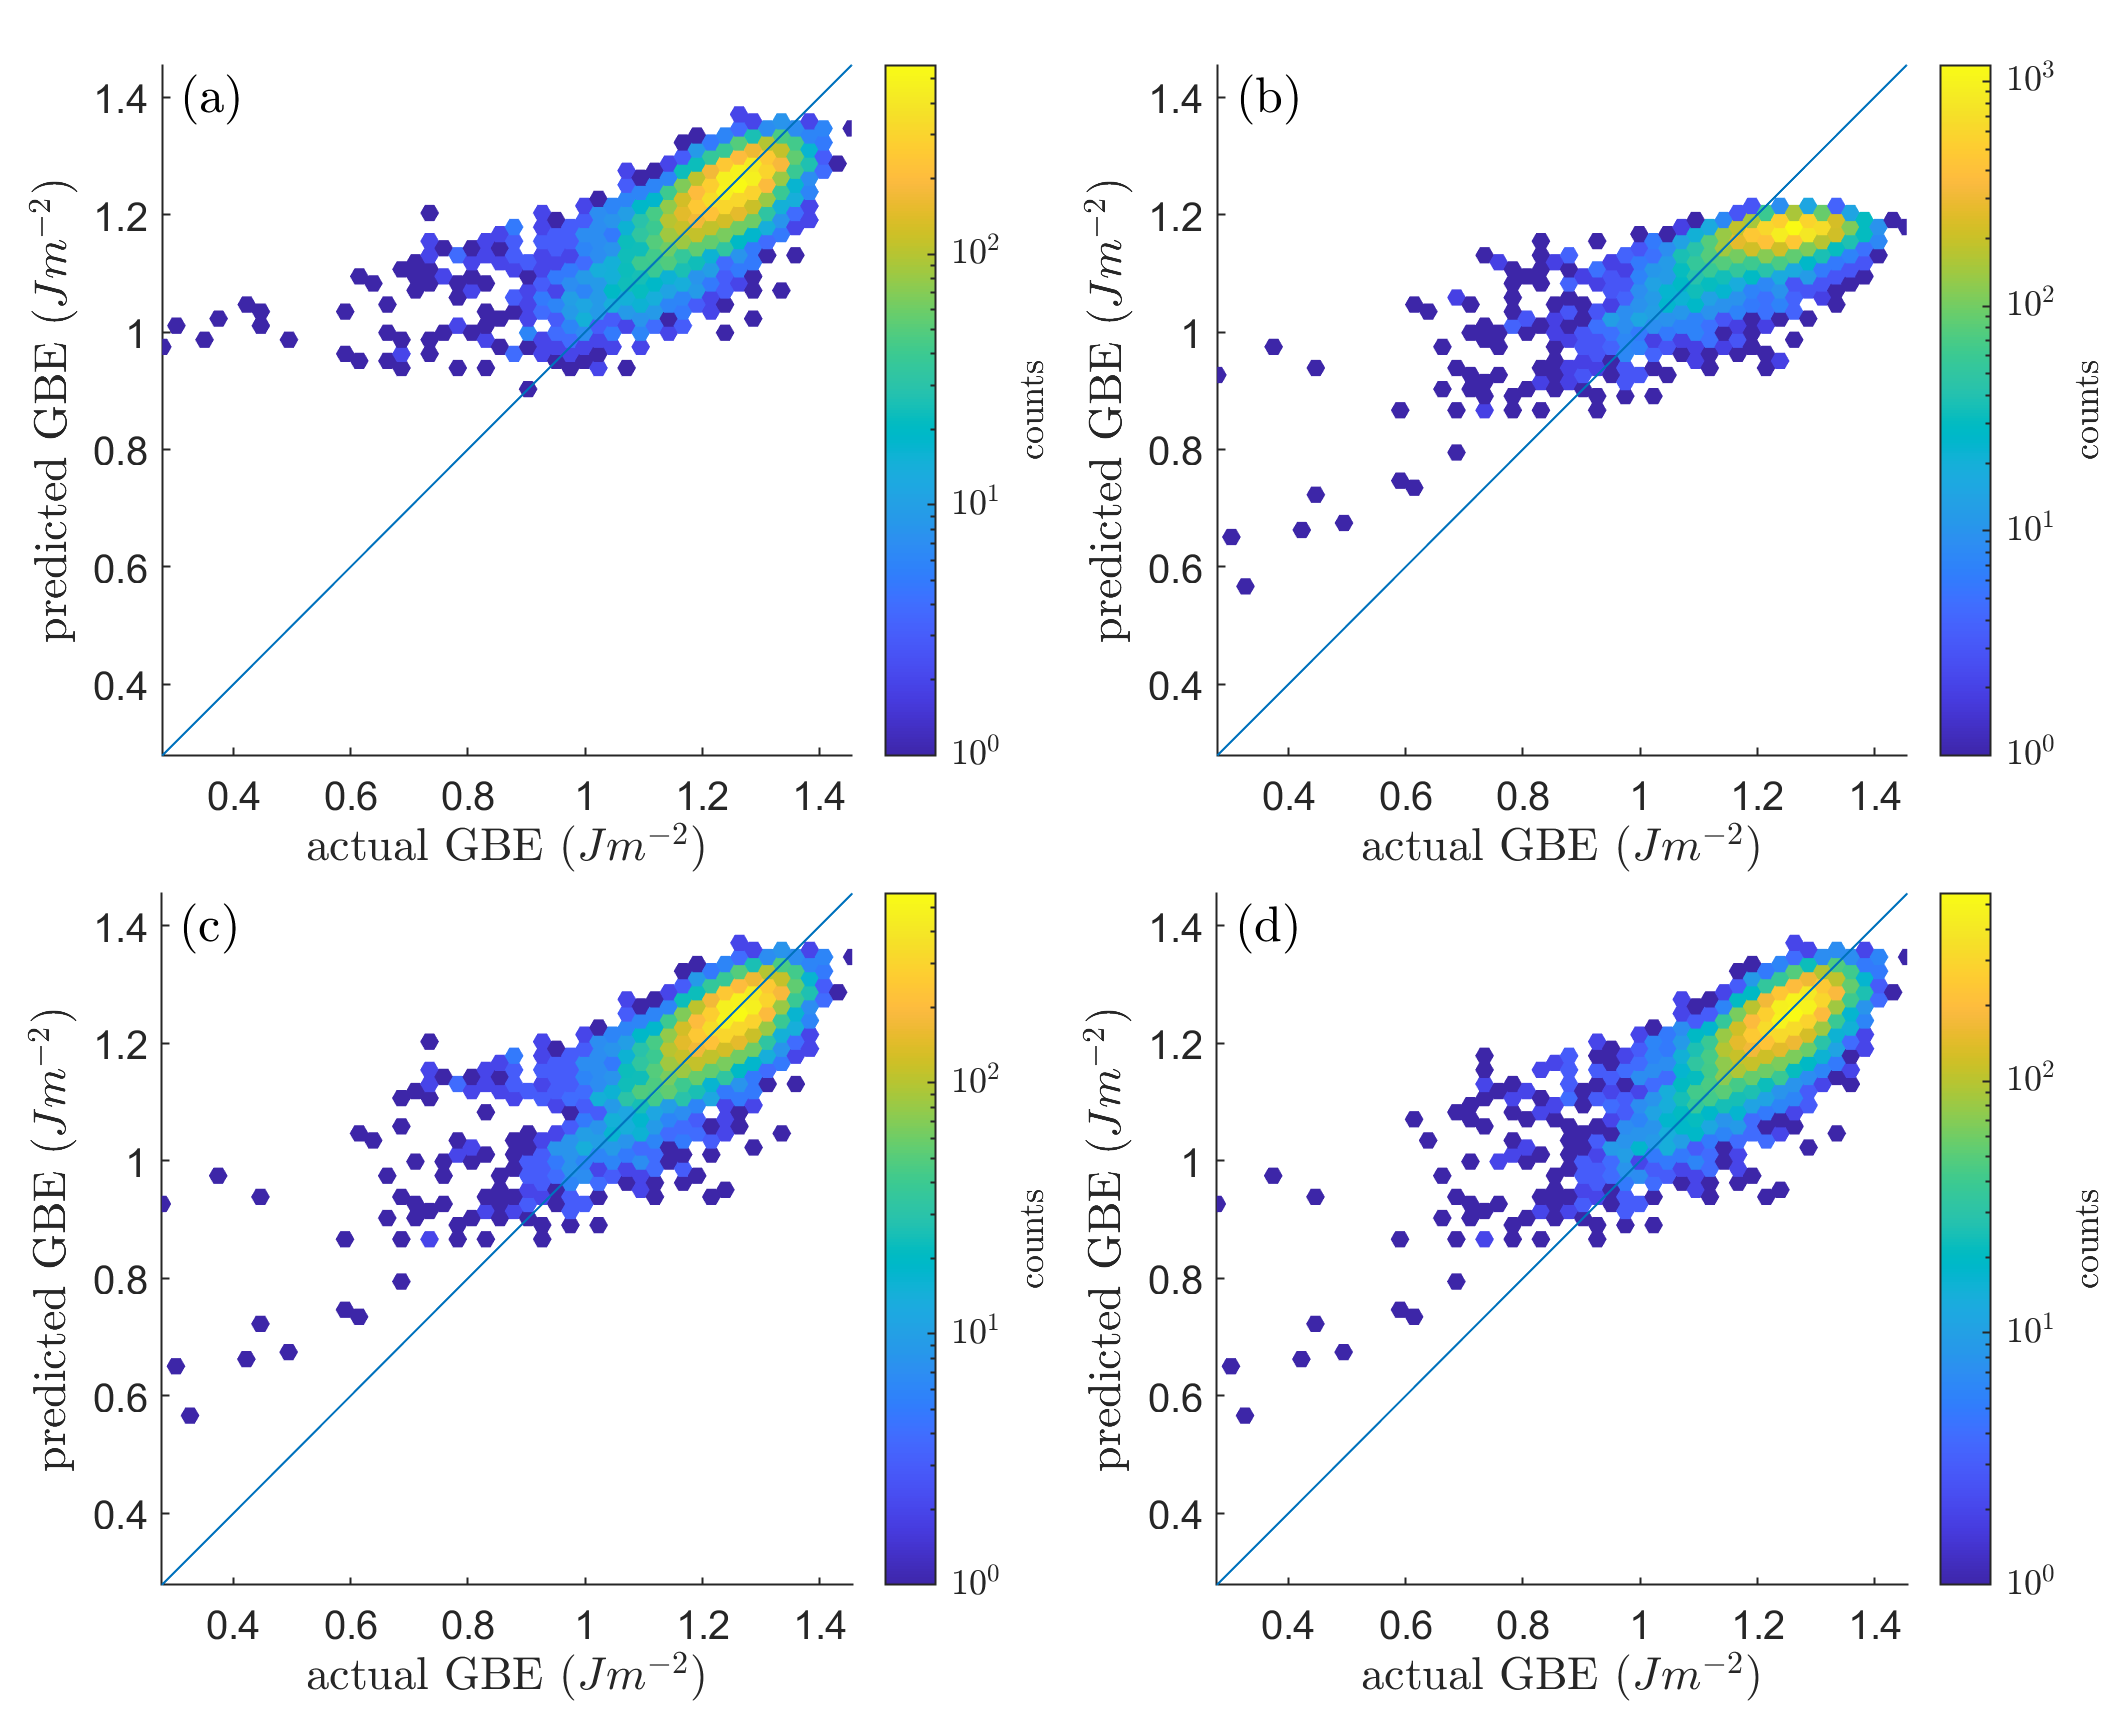
\includegraphics[scale=1]{kim-interp-teach.png}
    \caption{(a) Hexagonally binned parity plot of the standard \gls{gpr} model. (b) All prediction \glspl{gb} based on the model using only training \glspl{gb} with a \gls{gbe} less than \thrtwo{}. (c) Combined disjoint model as explained in the text. (d) Hexagonally binned parity plots of the final \gls{gpr} mixing model. Points in (c) are produced by splitting the prediction data into less than and greater than \thr{}. A sigmoid mixing function (\cref{fig:gprmix-sigmoid}) is then applied where the predicted \glspl{gbe} shown in (c) determines the mixing fraction ($f$) to produce a weighted average of models (a) and (b). A large Fe simulation database \cite{kimPhasefieldModeling3D2014} using \num{46883} training datapoints and \num{11721} validation datapoints in an 80\%/20\% split. The \gls{gpr} mixture model decreases error for low \gls{gbe} and changes overall \gls{rmse} and \gls{mae} from \SI{0.056868}{\J\per\square\meter} and \SI{0.039201}{\J\per\square\meter} in the original model (shown in (a)) to \SI{0.054085}{\J\per\square\meter} and \SI{0.038599}{\J\per\square\meter} (shown in (d)), respectively.}
    \label{fig:kim-interp-teach}
\end{figure}

A combined, disjoint model (\cref{fig:kim-interp-teach}c) is taken ($\epsilon_3$) by replacing $\epsilon_1$ \gls{gbe} predictions for \glspl{gb} with \gls{gbe} less than \thr{} with the corresponding $\epsilon_2$ predictions. Finally, a weighted average (\cref{eq:gprmix}) is taken according to:

\begin{equation}
    \epsilon_{mix} = f \epsilon_1+(f-1) \epsilon_2
    \label{eq:gprmix}
\end{equation}
where $\epsilon_1$ and $\epsilon_2$ represent the standard \gls{gpr} model and the \gls{gpr} model trained on the subset of \glspl{gb} with a \gls{gbe} less than \thrtwo{}, respectively, and $f$ is the sigmoid mixing fraction given by:

\begin{equation}
    f=\frac{1}{e^{-m \left(\epsilon_3-b\right)}+1}
        % f\left(\epsilon_3\right)=\frac{1}{e^{-m \left(\epsilon_3-b\right)}+1}
    \label{eq:sigmoid}
\end{equation}
and shown in \cref{fig:gprmix-sigmoid} with $m=30$ and $b=\sigthr{}$, as used in this work. Larger values of $m$ yield a steeper sigmoid function and larger values of $b$ shift the sigmoid function further to the right. Specific values for $m$ and $b$ were chosen by visual inspection and trial and error. This results in a \gls{gpr} mixing model which better predicts low \glspl{gbe} while retaining overall predictive accuracy (\cref{fig:kim-interp-teach}d).

\begin{figure}
    \centering
    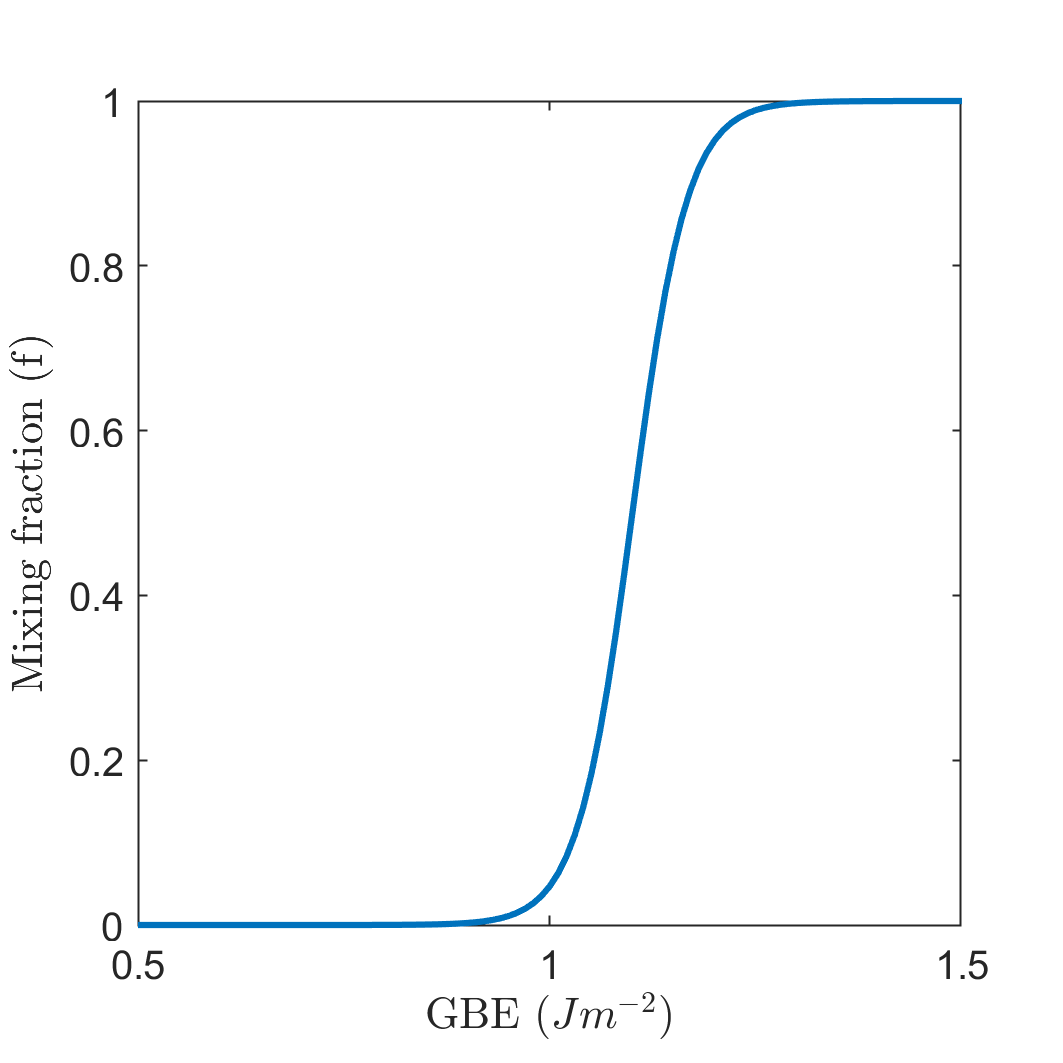
\includegraphics[scale=1]{figures/gprmix-sigmoid.png}
    \caption{Sigmoid mixing function used in the \gls{gpr} mixing model with $m=30$ and $b=\sigthr{}$ (\cref{eq:sigmoid}).}
    \label{fig:gprmix-sigmoid}
\end{figure}

Uncertainty of the \gls{gpr} mixing model is similarly obtained by taking a weighted average of the uncertainties of each model according to:

\begin{equation}
    \sigma_{mix} = f \sigma_1+(f-1) \sigma_2
    \label{eq:gprmix-sigma}
\end{equation}
where $\sigma_1$ and $\sigma_2$ are the corresponding uncertainties of $\epsilon_1$ and $\epsilon_2$, respectively, and $f$ is given by \cref{eq:sigmoid}. 

\section{Olmsted Interpolation}

As illustrated in \cref{fig:olmsted-Ni-loocv}, \gls{loocv} interpolation results for \SI{0}{\kelvin} \gls{ms} low-noise Ni simulations using the \gls{gpr} method are similar to \gls{lkr} results reported in Figure 6a of \citet{chesserLearningGrainBoundary2020} (reproduced on the right of \cref{fig:olmsted-Ni-loocv} for convenience).

\begin{figure}
     \centering
     \begin{subfigure}[b]{0.5\textwidth}
         \centering
         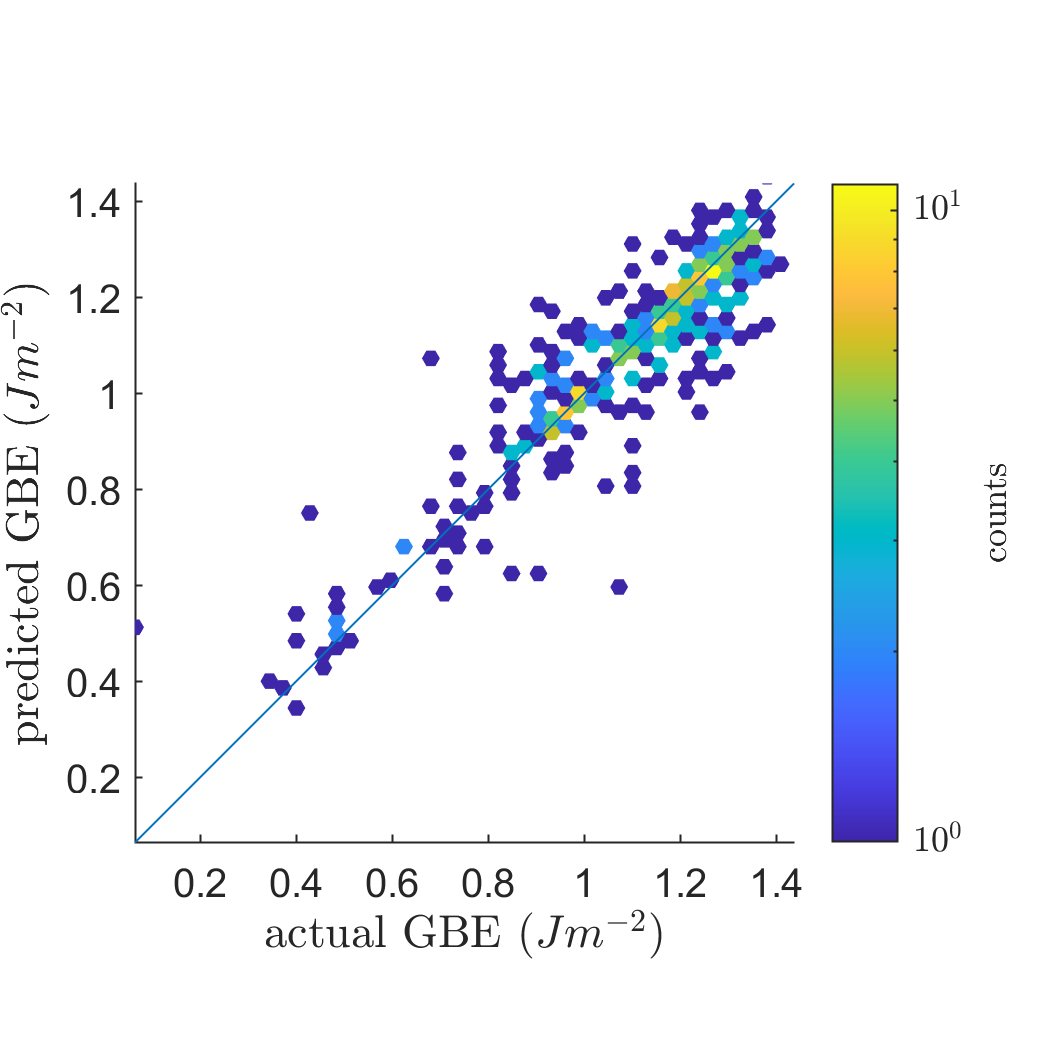
\includegraphics[width=\textwidth]{figures/olmsted-Ni-loocv.png}
        %  \caption{}
         \label{fig:our-loocv}
     \hfill
     \end{subfigure}
          \begin{subfigure}[b]{0.4\textwidth}
         \centering
         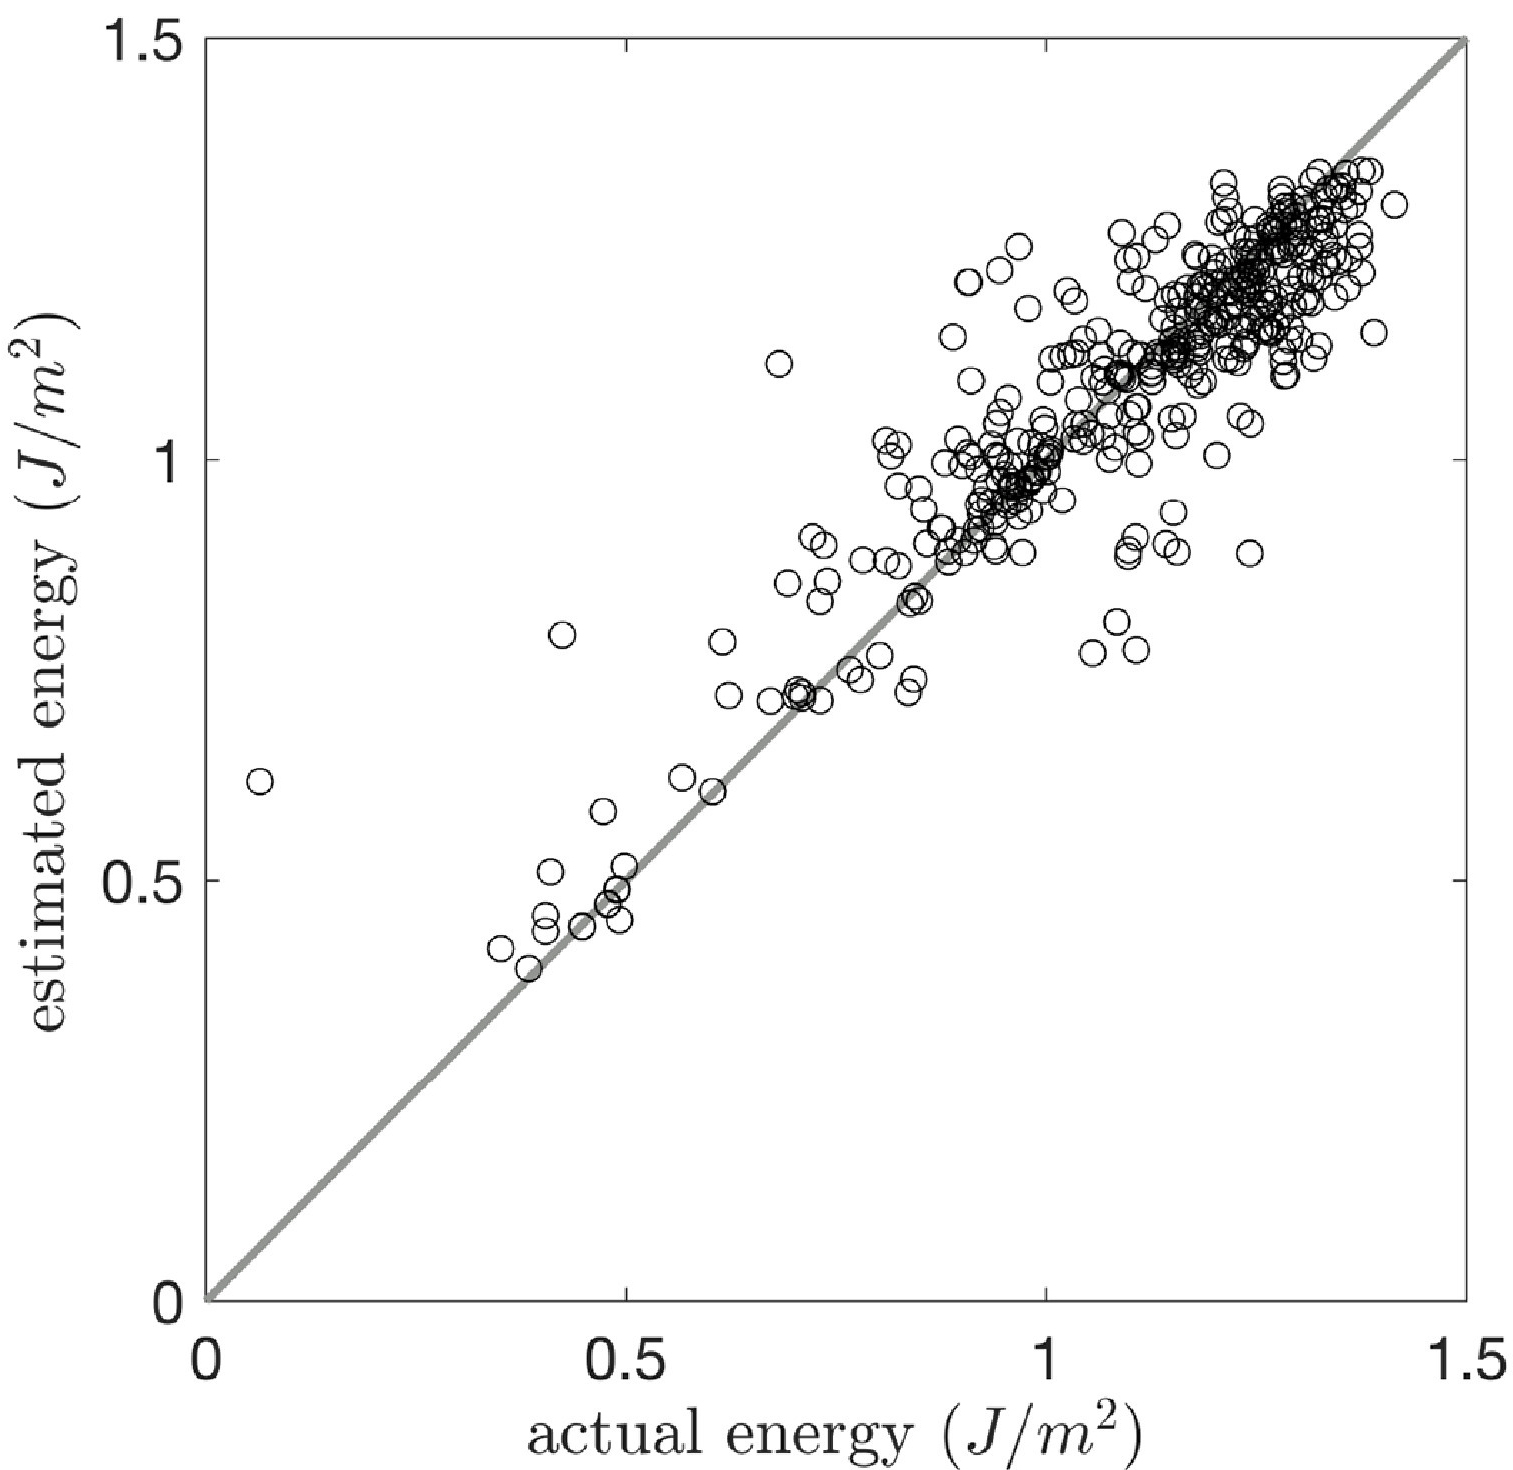
\includegraphics[width=\textwidth]{figures/ChesserFigure.jpg}
        %  \caption{}
         \label{fig:chesser-loocv}
     \end{subfigure}
        \caption{(left) Hexagonally binned parity plot for Ni simulation \glsxtrfull{gbe} interpolation using \glsxtrshort{loocv}. (right) Parity plot for \glsxtrfull{loocv} interpolation results reproduced from Figure 6a of \citet{chesserLearningGrainBoundary2020} under CC-BY Creative Commons license. }
        \label{fig:olmsted-Ni-loocv}
\end{figure}

% \begin{figure}
%     \centering
%     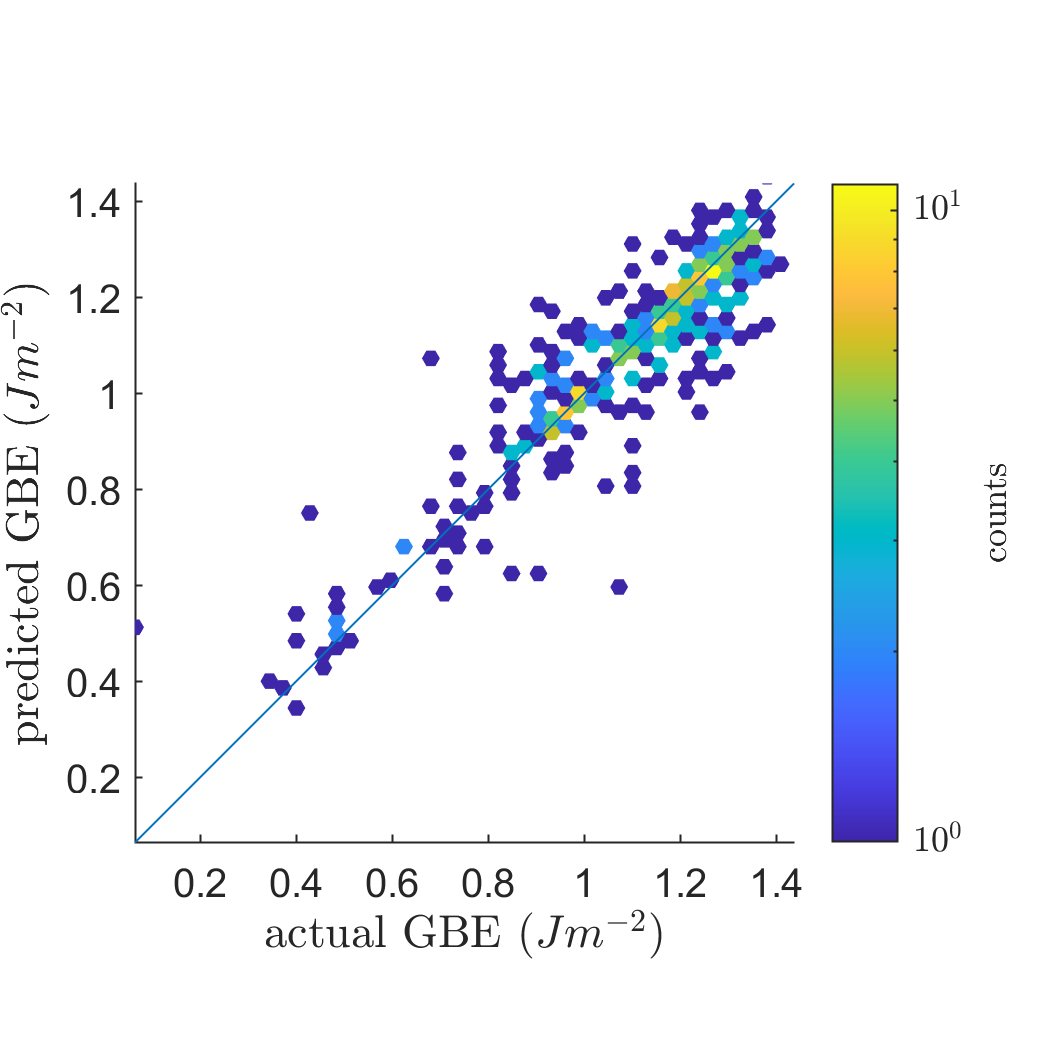
\includegraphics{figures/olmsted-Ni-loocv.png}
%     \caption{Hexagonally binned parity plot for Ni simulation \glsxtrfull{gbe} interpolation using \glsxtrfull{loocv}. }
%     \label{fig:olmsted-Ni-loocv}
% \end{figure}

%The true, underlying \gls{brk} function is also shown (black line) and a shaded error band of uncertainty standard deviation. \glspl{knn} ($1<=k<=6$) \inpt{} points closest to $\overline{AB}$ are plotted and colored by distance to $\overline{AB}$.

\newpage
\clearpage %make sure figures don't go past glossaries, bibliography, etc.
\printglossary[title={List of Acronyms}]
%need to manually clear cached files & logs in overleaf to get updated abbreviations to appear

\newpage
\bibliographystyle{elsarticle-num-names}
\bibliography{5dof-gb-energy.bib}

\end{document}